\documentclass[12pt,a4paper,twoside]{book}
\usepackage[utf8]{inputenc}
\usepackage{amsmath}
\usepackage{amsfonts}
\usepackage{amssymb}
\usepackage{graphicx}
\usepackage[inner=3.00cm, outer=2.50cm, top=3.00cm, bottom=3.00cm]{geometry}
\usepackage[slovene]{babel}
\usepackage{babelbib}
\usepackage{titlesec}
\usepackage{listings}
\usepackage{pdfpages}
\usepackage{fancyhdr}
\usepackage{eurosym}
\usepackage{url}
\author{Luka Horvat}
\title{Dobre prakse pri razvoju računalniških iger}

\graphicspath{{images/}}
%Paragraph indenting, title spacing and line spacing
\setlength{\parindent}{0pt}
\setlength{\parskip}{1em}
\renewcommand{\baselinestretch}{1.5}

% Remove big chapter text
\titleformat{\chapter}{\bfseries\LARGE}{\thechapter}{1em}{\LARGE\textbf}

% Code listings
\lstdefinestyle{mystyle}{
	numbers=left,
	breaklines=true,
	basicstyle=\footnotesize,
	frame=tb,
	captionpos=b
}
\lstset{style=mystyle}
\renewcommand{\lstlistingname}{Izsek kode}
\renewcommand{\lstlistlistingname}{Seznam izsekov kode}
%\renewcommand{\thelstlisting}{\thesection.\arabic{lstlisting}}

%Header/footer
\pagestyle{fancy}
\fancyhf{}
\fancyfoot[LE, RO]{\thepage}
\renewcommand{\headrulewidth}{0pt}
\renewcommand{\footrulewidth}{0pt}

\fancypagestyle{plain}{%
	\fancyhf{}
	\renewcommand{\headrulewidth}{0pt}
	\fancyfoot[LE, RO]{\thepage}
}

%Initial pages are in Roman numbering
\pagenumbering{Roman}
\begin{document}
	
%First page
\thispagestyle{empty} 
\begin{center}
	{\large 
		UNIVERZA V MARIBORU\\
		FAKULTETA ZA ELEKTROTEHNIKO,\\
		RAČUNALNIŠTVO IN INFORMATIKO\\
	}
	
	\vspace{\fill}
	{\LARGE Luka Horvat}\\
	
	\vspace{1cm}
	\textsc{\textbf{\LARGE DOBRE PRAKSE PRI RAZVOJU RAČUNALNIŠKIH IGER\\}}
	
	\vspace{1cm}
	{\LARGE Magistrsko delo}
	
	\vfill
	{\Large Maribor, julij 2018}
	\newpage
\end{center}

%Empty page
\ \thispagestyle{empty}
\newpage

%Second page
\thispagestyle{empty} 
\begin{center}	
	\vspace*{\fill}
	\textsc{\textbf{\LARGE
			Dobre prakse pri razvoju računalniških iger\\
	}}
	{\large\textbf{Magistrsko delo\\}
		
	}
	\vspace{\fill}
	\begin{tabbing}
		\hspace*{4cm}\=\hspace*{3cm}\= \kill
		Študent: \> Luka Horvat\\
		Študijski program: \> Študijski program 2. stopnje\\
		\>Računalništvo in informacijske tehnologije\\
		Mentor: \> doc. dr. Matej Črepinšek
	\end{tabbing}
\end{center}
\newpage

%Empty page
\ \thispagestyle{empty}
\newpage

%%% ZAHVALA (NEOBVEZNO)

\mbox{}
{\raggedleft\vfill\itshape%
		\textbf{Zahvala}\\
		Zahvaljujem se svojemu mentorju \\za ves čas in trud, ki ga je vložil \\za pomoč pri izdelavi magistrskega dela. \\
		Zahvalil bi se rad tudi moji družini,\\ki me je podpirala skozi vsa študijska leta.  \\
	}\par

%Empty page
\ \thispagestyle{empty}
\newpage
\ \thispagestyle{empty}
%Povzetek v slovenskem jeziku
\chapter*{Dobre prakse pri razvoju računalniških iger}\thispagestyle{fancy}
\setcounter{page}{1}
\textbf{Ključne besede:} računalniška igra, metode, prakse, RayLib, LibGDX, Unity

\textbf{UDK:} 004.388.4:004.42(043.2)

\textbf{Povzetek}\newline
\textit{Magistrsko delo predstavi metode in prakse, potrebne za razvoj računalniških iger. Najprej opišemo orodja, ki so nam na voljo od samega začetka koncipiranja do konca razvoja. Zatem se posvetimo tehnični implementaciji in dokumentaciji ustaljenih metod ter praks v treh orodjih: RayLib, LibGDX in pogon Unity. Za potrebo demonstracij opisanih metod implementiramo igro Breakout v vseh treh orodjih in končni izdelek tudi opišemo.}
\cleardoublepage

%Povzetek v angleškem jeziku
\chapter*{Good practices for computer game development}\thispagestyle{fancy}
\textbf{Key words:} computer game, practices, RayLib, LibGDX, Unity

\textbf{UDK:} 004.388.4:004.42(043.2)

\textbf{Abstract:}\newline
\textit{The thesis focuses on demonstrating good practices required for game development. We first introduce the different tools that are available to us from the start of development till the end. After that, we focus on the technical implementation and documentation of the standard practices using three different tools: RayLib, LibGDX and Unity engine. For the purpose of demonstrating the documented practices, we also implement the game Breakout in all three tools and document the final product in the end.}
\cleardoublepage

%Kazalo
\tableofcontents

%Kazalo vsebine
\listoffigures

%Kazalo kode
\lstlistoflistings

%Seznam kratic
\chapter*{Seznam uporabljenih simbolov in kratic}\thispagestyle{fancy}
\begin{itemize}
	\item 2D - dva dimenzionalno
	\item 3D - tri dimenzionalno
	\item SGC - Slovenian Games Conference
	\item SDK - Software Development Kit
	\item SVN - Apache Subversion
	\item LMMS - Linux MultiMedia Studio
	\item SDL - Simple DirectMedia Layer
	\item GLFW - Graphics Library Framework
	\item BMP - Bitmap
	\item GIF - Graphics Interchange Format
	\item JPEG - Joint Photographic Experts Group
	\item PNG - Portable Network Graphics
	\item SVG - Scalable Vector Graphics
	\item FLAC - Free Lossless Audio Codec
	\item MIDI - Musical Instrument Digital Interface
	\item SOIL - Simple OpenGL Image Library
	\item TTF - TrueType Font
	\item TCP - Transmission Control Protocol
	\item UDP - User Datagram Protocol
	\item RTF - Rich Text Format
	\item VR - Virtual Reality
	\item XNA - XNA's not acronymed
	\item JS - JavaScript
	\item MIT - Massachusetts Institute of Technology
	\item GUI - Graphical User Interface
\end{itemize}
%Content
%Uvod
\chapter{Uvod}\thispagestyle{fancy}
%Page numbering and style changes here
\setcounter{page}{1}
\pagenumbering{arabic}

Računalniške igre so ena izmed panog v zabaviščni industriji. Skozi leta se njihov delež samo povečuje. Dandanes se je že skoraj vsak posameznik srečal z računalniškimi igrami. Ali neposredno z igranjem v prostem času, ali pa so se posredno vključile v kulturo okrog posameznika. Računalniške igre in še posebej like iz njih velikokrat vidimo v drugih medijih, kot so filmi, serije, oglasi ter tiskano gradivo. Kdo pa si danes pod imenom Mario ne predstavlja vodovodarja z velikimi brki v rdečem kombinezonu?

Računalniške igre privabljajo vedno več podjetij in individualnih razvijalcev, ki poskušajo zavzeti svoj prostor v tej industriji. Samo izdelovanje računalniških iger uvrščamo pod razvoj programske opreme, ki je izredno kompleksen in zahteva znanja iz različnih panog. Napredek tehnologije pa je že skoraj vsakemu posamezniku omogočil preprost vstop v ta proces. Dandanes je na voljo veliko različnih orodij, knjig, procesov in ustaljenih praks, ki so posamezniku na voljo, vendar se v oceanu podatkov hitro izgubijo. Tako smo si kot cilj tega magistrskega dela zadali poiskati, opisati in preizkusiti dobre ter priporočene prakse pri razvoju računalniških iger. Zajeli smo celoten spekter procesa, od same začetne ideje do izdaje igre na trg. Večji del magistrskega dela smo posvetili bolj tehnološko usmerjenim procesom pri izdelavi računalniške igre, pri čemer smo prikazali različna orodja in prakse, ki so dandanes na voljo.

Magistrsko delo sestoji iz štirih poglavij. Prvo poglavje je uvod. V drugem poglavju predstavimo glavne korake, ki so potrebni pri razvoju računalniških iger. V tretjem poglavju opišemo orodja, ki so nam na voljo skozi proces razvoja iger, od načrtovanja in vodenja razvoja do končne tehnične implementacije. V četrtem poglavju se osredotočimo na tehnično implementacijo računalniških iger. Predstavimo dobre ustaljene prakse, ki se uporabljajo v razvoju. Metode opišemo, dokumentiramo in implementiramo v treh različnih orodjih: RayLib, LibGDX in pogon Unity. Za potrebe demonstracije metod implementiramo v vseh treh orodjih igro Breakout.

%Main content
\chapter{Pregled in opis razvoja}\thispagestyle{fancy}
V tem poglavju smo opisali osnovno problematiko razvoja igre, kot so sodelujoče vloge, metode koncipiranja, postopek izdelave, marketing ter možnosti izdaje.
\section{Opis problema}
\label{sec:opis_problema}
Razvoj računalniških iger je proces razvoja programske opreme. Obenem je kreativen proces, v katerem sodeluje širok spekter ljudi iz različnih panog. Glavne vloge v tem procesu so \cite{rogers2014level}:
\begin{itemize}
	\item \textbf{Programer (angl. \textit{programmer}):} je odgovoren za tehnično implementacijo računalniške igre. Odvisno od velikosti projekta in končnega cilja uporablja obstoječe namenske pogone za razvoj računalniških iger (npr. Unity ali Unreal Engine) ali implementira \textit{"in-house"} pogon za to specifično igro. Tukaj pridejo v poštev različna znanja iz 2D in 3D grafike, fizike, umetne inteligence, uporabniških vmesnikov, računalniških mrež ipd. Obenem je potreben še ves spekter računalniškega znanja, ki se navezuje na principe, specifične za računalniške igre.
	\item \textbf{Umetnik (angl. \textit{artist}):} je odgovoren za izdelavo vseh grafičnih gradnikov. Določeni umetniki izrisujejo samo konceptne slike in z oblikovalcem poskusijo definirati končni cilj igre, kako bo videz igre, kakšni bodo glavni liki ipd. Preostali umetniki pripravljajo gradnike, ki se nato uporabijo v sami računalniški igri. To so lahko grafični gradniki za menije, 3D modeli objektov, teksture za omenjene modele, vizualni efekti, animacije ipd.
	\item \textbf{Oblikovalec (angl. \textit{designer}):} je odgovoren za koncipiranje in definiranje računalniške igre. Išče in definira ideje, ki so in bodo pomembne za igro. Pomembna vrlina je, da je zmožen te ideje dobro predstaviti preostali ekipi, da jo ta potem uresniči. Določeni oblikovalci se lahko osredotočijo na specifične dele igre, kot so stopnje v igri in določeni sistemi (npr. sistem bojevanja).
	Specifična panoga oblikovalca je tudi pisatelj, ki je odgovoren za zgodbo v igri. Včasih je sama zgodba rdeča nit in je glavna gonilna sila za nastanek igre, drugič pa se zgodba komaj oblikuje skozi nastanek končnega produkta.
	\item \textbf{Skladatelj in oblikovalec zvoka (angl. \textit{composer and sound designer}):} je odgovoren za vse zvočne gradnike igre. Skladatelji pripravljajo glasbo v igri. Dandanes pri večjih projektih sodelujejo tudi celotni orkestri. Oblikovalec zvoka pa je odgovoren za različne krajše zvoke, ki se prožijo ob določenih akcijah (npr. streli orožij).
	\item \textbf{Preizkuševalec (angl. \textit{tester}):} testira produkt skozi vse faze razvoja in daje povratne informacije drugim razvijalcem za izboljšanje produkta. Zagotavlja kakovost igre, da bo ta izšla brez hujših napak.
\end{itemize}
Poleg naštetih, je na področju izdajanja igre še veliko drugih vlog, kot so vodenje ekipe, marketinga ipd., vendar so zgoraj naštete najbolj pomembne pri samem razvoju igre. Znanja, ki jih te vloge premorejo, so pomembna za razvoj vsake igre. Če gre za večji projekt, potem je za posamezno vlogo potrebnih več ljudi. Dandanes pri velikih podjetjih pri razvoju iger sodeluje preko sto ljudi. Na trgu pa obstaja tudi velika scena individualnih razvijalcev (angl. \textit{indie developer}), ki sami nastopijo v večini vlog in tako uresničijo svoje projekte. 

V tem magistrskem delu smo se posvetili individualnemu razvoju računalniške igre in praksam, ki temu pristopu najbolj ustrezajo. Kot posamezni razvijalec je potrebno uporabiti znanja iz različnih panog, zato smo s tem delom poskusili zaobjeti prakse, ki bi ta proces olajšale. V delu smo našteli in opisali različna orodja ter procese za vsak korak v razvoju. Glavni koraki razvoja so sledeči: koncipiranje in definiranje igre, planiranje in vodenje dela, tehnični razvoj igre (pri tem pride v poštev izdelava grafičnih in zvočnih gradnikov ter implementacija), oglaševanje in viri občinstva ter na koncu izdaja igre.

\section{Koncipiranje igre}
V prvem koraku razvoja igre je potrebno definirati, kaj želimo ustvariti. Ta korak opravlja oblikovalec igre. Lahko, da ima svojo sanjsko idejo, ki jo hoče uresničiti. Drugim se nenadoma prikrade ideja, ki jo potem razvijejo v delujoč produkt. Velikokrat pa je potrebno vložiti delo, da definiramo originalno idejo igre. Studii, katerim je razvoj iger glavni vir prihodka, se ne morejo zanašati na naključne ideje. Obenem je izvirna in dobro premišljena ideja pomembna, če hočemo kot individualna oseba razviti svojo igro, saj je trg danes zelo nasičen in je prvi vtis zelo pomemben. Spodaj smo našteli nekaj načinov, kako spodbuditi ustvarjalnost in poiskati novo idejo za igro \cite{rogers2014level}: 
\begin{itemize}
	\item \textbf{Igranje obstoječe (slabe) igre.} Igre konstantno gradijo na idejah in mehanikah obstoječih iger. Dodajajo se novi koncepti in pravila, ki iz starih idej zgradijo nove izkušnje. Za vsako komercialno igro se lahko našteje ducat drugih, ki so služile kot navdih in podlaga za njo. Tako je dober način za iskanje idej igranje že obstoječih iger. Še boljše je igranje slabih iger in razmislek, kaj bi spremenili, da bi izkušnjo izboljšali. Tako iteriramo na obstoječih rešitvah, da definiramo nekaj boljšega.
	\item \textbf{Branje tematike izven osebnega zanimanja.} Razširjanje osebnega obzorja, znanja in izkušenj je vedno dober vir novih idej. Velikokrat je pri igrah problem, da so si preveč podobne. Dandanes se zelo pogosto dogaja, da vsi poskusijo kopirati idejo iz nove, uspešne igre. Zato je pomembno, da raziščemo tematike, ki jih ne poznamo najbolje in poskusimo tam najti nove ideje.
	\item \textbf{Udeleževanje konferenc in predavanj.} Konference so vedno polne različnih ljudi z novimi idejami. V takem okolju hitro najdemo inspiracijo, ki jo lahko izkoristimo za razvoj nove igre.
	\item \textbf{Viharjenje možganov (angl. \textit{brainstorming})}. Uveljavljena praksa iskanja novih idej. Pomembno je, da zberemo ljudi iz različnih področij in se držimo glavnega pravila: poudarek je na količini idej, ki se ne obsojajo \cite{osborn1953applied}. Tako poskusimo raziskati čim več idej, ki so lahko prvotno neprimerne in na teh nato gradimo vedno boljše rešitve.
\end{itemize}
Pri iskanju idej je pomembno, da se zavedamo svojih omejitev. Če smo posameznik, ki hoče uresničiti svojo prvo igro, potem je priporočljivo, da začnemo s preprostimi idejami. Take igre lahko potem uresničimo in postopoma povečujemo obsežnost naslednjih iger. Veliko posameznikov namreč začne s preveč ambicioznimi idejami, ko pa je potrebno projekt dejansko uresničiti, pa pride do komplikacij in pogosto do preliminarne zaključitve projekta \cite{ambitious1}\cite{ambitious2}\cite{ambitious3}.
\section{Potek razvoja igre}
Razvoj igre skoraj vedno poteka po določenih korakih, neodvisno od ideje. Glavni mejniki procesa so \cite{jainGameDevelopmentCycle}:
\begin{figure}[h]
	\centering
	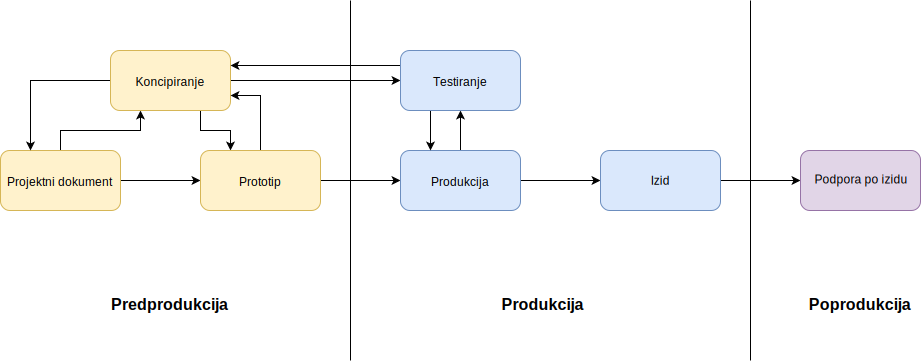
\includegraphics[width=15cm]{LifeCycle}
	\caption{Koraki razvoja igre}
	\label{slika:lifeCycle}
	\vspace*{-2em}
\end{figure}
\begin{enumerate}
	\item \textbf{Projektni dokument}. Tukaj preide ideja iz glave na fizični medij. Proces je zelo odvisen od velikosti projekta in studia. Pri večjih projektih nastane dokument, v katerem se definira ideja, kakšna bo mehanika igre, zgodba, liki, razporeditev sredstev, predviden čas izdelave ipd. Dokument je velikokrat opremljen tudi s konceptnimi slikami, ki jih pripravijo umetniki. S tem dokumentom je potem najlažje predstaviti vizijo preostalim ljudem v ekipi. Pri manjših idejah in posameznikih je ta korak bolj direkten. Ustvarijo se skice in krajši opisi, a se večinoma ta korak preskoči in je večji poudarek na prototipu.
	\item \textbf{Prototip}. Je najpomembnejši korak v procesu razvoja igre. Sama definicija besede prototip pomeni razvoj osnovnega produkta, ki je ustvarjen z namenom testiranja koncepta \cite{blackwell2015prototype}. Glavni namen je preizkusiti, ali je glavna ideja igre dovolj dobra, da iz nje nastane končni produkt. Prototipiranje je zelo povezano s samim koncipiranjem in projektnim dokumentom. Pri tem se identificirajo pomanjkljivosti, ki jih je potrebno razčistiti in mogoče znova koncipirati, ter prednosti, ki jih je potrebno poudariti v končnem produktu. Dober prototip je odločilen mejnik v razvoju, ki se uporablja kot izhodiščna točka za začetek pravega projekta. Obenem služi kot prikaz koncepta možnim investitorjem, ki bi hoteli vložiti v projekt. 
	\item \textbf{Produkcija}. Je glavni del razvoja projekta. Sodelujejo vsi člani ekipe, opisani v poglavju \ref{sec:opis_problema}. Konstantna komunikacija med razvijalci, preizkuševalci in oblikovalci pelje projekt skozi faze razvoja programske opreme: \textit{pre-alpha, alpha, beta, release candidate, live release (gold)}. Odvisno od projekta se lahko studio odloči, da izdajo produkt končnim uporabnikom še v fazi razvoja. Tako postanejo uporabniki del preizkuševalcev, ki pomagajo pri razvoju projekta.
	\item \textbf{Izid}. Pomeni konec glavnega procesa razvoja. Igra se zapakira in distribuira do končnih uporabnikov preko posrednikov. Ker mine kar nekaj časa od verzije, ki jo razvijalci dajo distribuirat, do dejanskega izida, je danes ustaljena praksa prenos popravkov preko spleta na dan izida. Nekoč se je na tej točki razvoj igre zaključil, razvijalci pa so prehajali na naslednji projekt. Dandanes pa izid pomeni le še en mejnik v samem življenjskem ciklu igre.
	\item \textbf{Podpora po izidu} . Tako imenovan \textit{post production} postaja danes vedno večji faktor. Razvoj igre je veliki finančni podvig, ki največ sredstev terja do izida igre. Zato se veliki studii raje posvetijo izdani igri z nadaljnjo podporo. Začel se je uporabljati termin igre kot storitev (angl. \textit{games as a service}). Studii podpirajo igro še vrsto let z novimi vsebinami, popravki ter včasih korenitimi spremembami s ciljem maksimirati dobiček. Konstantna komunikacija s ciljno publiko je pomembna, saj tako identificirajo, kaj si igralci želijo novega v igri.
\end{enumerate}
Zgornji koraki so razvidni s sliki \ref{slika:lifeCycle}. Vidimo, da je proces razvoja, testiranja in koncipiranja zelo povezan, saj se igra nenehno izboljšuje.

\section{Marketing}
Uspešna izdaja računalniške igre je zelo odvisna od marketinga pred izidom. Brez marketinga je zelo težko, da bo kdo našo igro opazil, kaj šele kupil. Samo na igralni platformi Steam letno izide več kot 6000 iger \cite{james6000Games}. V tej množici je pomembno, da naša igra izstopa in prav tukaj je zelo pomemben marketing že v zgodnjih fazah razvoja. Dober čas, da začnemo z marketingom, je, ko lahko pokažemo glavne koncepte igre. Velikokrat so to slike ali videi igre v gibanju, ki pritegnejo končnega uporabnika \cite{robertMarketing}.

Obstaja veliko različnih načinov marketinga. Spodaj našteti so dandanes že skoraj obvezni, če hočemo uspeti na trgu \cite{robertMarketing}:
\begin{itemize}
	\item \textbf{Spletna stran.} Vsaka igra potrebuje svojo spletno stran. Brez te bo končna publika težko našla dodatne informacije o igri. Pomembno je, da stran vestno posodabljamo z opisom koncepta igre, s slikami, videi ipd. Ena možnost za hitro postavitev strani je orodje \textit{presskit()} \footnote{http://dopresskit.com/}, prosto dostopen paket za enostavno izdelavo strani računalniške igre.
	\item \textbf{Blog.} Dober vir marketinga in občinstva je blog, kjer opisujemo potek razvoja igre. Veliko igralcev zanima, kako poteka razvoj in v katerem stanju se igra trenutno nahaja. Je tudi dober vir povezovanja z drugimi razvijalci, ki bi jih mogoče zanimalo sodelovanje na projektu. Paziti moramo le, da ne pretiravamo z objavami, saj ni vsak napredek v razvoju vreden omembe.
	\item \textbf{Družabni mediji.} Dandanes skoraj največja možnost pridobitve ciljnega občinstva so družabni mediji. Dobra promocija igre na Facebooku in kratke zanimive objave na Twitterju lahko doprinesejo veliko. Družabna omrežja ponujajo tudi svoj plačljiv marketing, s katerim lahko ciljamo specifično publiko, ki bi se zanimala za našo igro.
	\item \textbf{Konference.} Vsako leto poteka več konferenc, kjer se razvijalci predstavijo s svojimi igrami. Na konferencah	se obrne veliko igralcev in različnih medijev, ki zelo pripomorejo k marketingu igre. Tri izmed večjih konferenc na to temo so Pax\footnote{http://www.paxsite.com/}, IndieCade\footnote{http://www.indiecade.com/} in Indie Mega Booth\footnote{http://indiemegabooth.com/}. V Sloveniji je največja konferenca SGC\footnote{http://sgc.si/}.
	\item \textbf{Množično financiranje (angl. \textit{crowdfunding}).} Danes vedno bolj priljubljen način zbiranja sredstev in občinstva za razvoj igre. Preko strani kot je Kickstarter predstavimo svojo vizijo in načrt razvoja ter tako poskusimo doseči igralce, ki bi jih zanimala naša igra. Ti lahko nato financirajo razvoj z upanjem, da bo končni produkt vreden njihove investicije.
	\item \textbf{Napovednik (angl. \textit{trailer}).} Ko se igra začne bližati zaključnim fazam razvoja, je dobro izdelati napovednik, ki se bo potem uporabil na platformah, kjer bomo igro izdali. V napovedniku je pomembno, da prikažemo glavni koncept igre in da smo iskreni o vsebini. Zavajajoči napovedniki lahko ustvarijo večjo začetno zanimanje, vendar po izidu hitro pritegnejo slabo kritiko.
\end{itemize}

\section{Možnosti izdaje igre}
Opisali smo nekaj možnosti, ki so nam na voljo za izdajo igre kot individualnemu razvijalcu. Večina teh možnosti predvideva, da nimamo svojega distributerja in so zato najbolj primerne za manjše projekte:
\begin{itemize}
	\item \textbf{Steam.} Največja platforma za digitalno distribucijo računalniških iger. Omogoča izgradnjo svoje strani za našo igro z vsemi potrebnimi informacijami. Sama platforma poskrbi za distribucijo, namestitev, posodobitve, varnostno kopijo shranjenih iger, glasovno komunikacijo v igri ipd. Na voljo je na vseh večjih operacijskih sistemih, kot so Windows, OSX in Linux. Če se odločimo, da bomo našo igro izdali na Steam platformi, nam Steam ponudi implementacijo njihovega SDK-ja, ki nudi proti-piratsko rešitev, mikro transakcije, oblačne storitve, dosežke ipd. Cena za izdajo igre je 100 evrov, provizija za vsako prodano kopijo igre pa je 30 \% \cite{steam}.
	\item \textbf{Itch.io.} Zelo priljubljena rešitev za individualne razvijalce, saj lahko svojo igro dodamo na njihovo platformo brezplačno. Podobno kot Steam ponujajo izgradnjo svoje strani za igro ter aplikacijo, ki skrbi za namestitve in posodobitve. Platforma ne ponuja svojega SDK, ki bi nudil dodatne funkcionalnosti. Možno je nastaviti minimalno ceno igre, kupci pa lahko po želji plačajo več. Provizija je 10 \% od vsakega nakupa, po želji pa lahko ta delež povečamo \cite{itchiofaq}.
	\item \textbf{Humble Bundle.} Ponuja tri vrste prodaje skozi njihovo platformo. Prva možnost je izgradnja brezplačne strani, kjer ponujamo svojo igro. Oni poskrbijo za transakcije in si vzamejo 5 \% provizije. Ta stran je neodvisna od njihove trgovine. Druga možnost je samostojen majhen gradnik, ki ga potem lahko dodamo na svojo spletno stran. Podobno kot pri njihovi neodvisni strani si vzamejo 5 \% provizije. Zadnja možnost pa je prodajanje na njihovi spletni trgovini. Tukaj lahko dobimo njihovo izpostavitev naše igre, imamo znižanja ipd. So samo spletna trgovina, ne ponujajo aplikacije za prenašanje in posodabljanje iger. Provizija za prodajo v njihovi trgovini je 25 \%, objava igre pa ne stane nič \cite{humblebundle}.
	\item \textbf{GameJolt.} Podobno kot itch.io je tudi GameJolt zelo priljubljena platforma za neodvisne razvijalce. Nudijo svojo aplikacijo za prenose in posodobitve. Objava igre v njihovi trgovini ne stane nič, provizija pa je 10 \% ali manj, saj ponujajo možnost znižanja provizije. Promovirajo skupnost neodvisnih razvijalcev, zato vse dobičke dobimo na njihov račun, ter jih lahko nato porabimo za nakup iger drugih razvijalcev, brez dodatne provizije. Seveda si je možno denar tudi izplačati \cite{gamejolt}.
	\item \textbf{Apple store in Google Play.} Če je naša igra namenjena za mobilne naprave, potem moramo obvezno uporabiti ti dve trgovini. Obe nudita izgradnjo svoje strani za igro na trgovini, prenose, posodobitve in dodatne transakcije. Kot mobilna platforma ponujata tudi dodatni SDK, s katerimi lahko v našo igro vgradimo lestvice, nagrade, oblačne storitve ipd. Provizija je 30 \% od nakupa, je pa potrebno plačati tudi za objavo aplikacije v trgovini. Pri Google Play je to enkratna cena 25 evrov, nakar lahko izdajamo neomejeno število aplikacij \cite{googleplay}. Pri Apple trgovini je cena 99 evrov na leto \cite{applestore}.
\end{itemize} 

\chapter{Orodja za izdelavo iger}\thispagestyle{fancy}
Razvoj iger ni mogoč brez nabora potrebnih orodjih v vseh fazah projekta. V tem poglavju smo nabrali in opisali različna orodja, ki so na voljo individualnim razvijalcem za brezplačno uporabo.
\section{Načrtovanje in vodenje razvoja}
Dobra organizacija veliko prispeva za tekoč razvoj računalniške igre. Obstaja veliko različnih orodij, nekatera so usmerjena v organizacijo ljudi in opravil, druga v organizacijo projekta in kode. Tudi, če samostojno razvijamo igro, nam ta orodja veliko pomagajo, zato smo poiskali dobre rešitve in jih tudi opisali.

\subsection{Organizacija ljudi in opravil}
Delo je priporočljivo razdeliti na manjša opravila, ki jih lahko opišemo, razdelimo med skupino in vodimo njihov napredek. Dve izmed boljših orodij za to sta Trello in HackNPlan. Obe pa uporabljata principe kanban razvojnega sistema.

\begin{figure}[h]
	\centering
	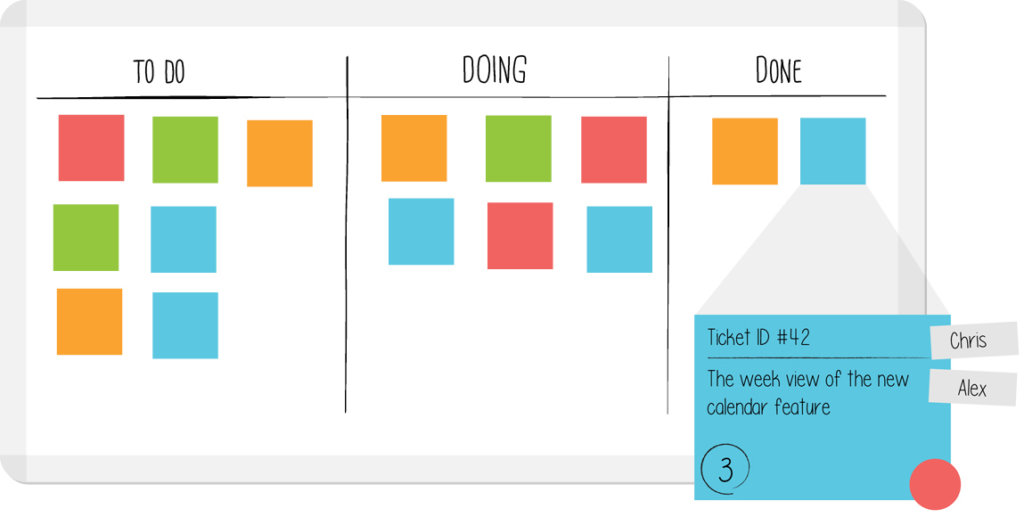
\includegraphics[width=10cm]{kanban_guide_print_KPO_bleed_board2}
	\caption{Kanban tabla. Vir \cite{kanbanBoard}}.
	\label{slika:kanbanBoard}
	\vspace*{-2em}
\end{figure}

Kanban sistem je način organizacije dela, katerega cilj je izboljšati ravnovesje med povpraševanjem in kapaciteto človeškega dela, ki je na voljo. Delo je razdeljeno na manjše kose in vizualizirano na kanban tabli, kot primer na sliki \ref{slika:kanbanBoard}. Opravila so večinoma vizualizirana na listkih, ki hranijo potrebne podatke, kot so naslov, opis, ocenjen čas potrebnega dela, trenutni upravitelji ipd. Ta opravila so uvrščena na pripadajoč del table, odvisno, v kakšnem stanju je opravilo (npr. čaka na dela, v razvoju, v testiranju, potrebno ocene, končano ipd.). Glavni cilj take organizacije je vizualizirati in kategorizirati opravila, ki jih nato razvijalci prevzamejo in opravijo \cite{kanbanBoard}.

Trello je produkt pod okriljem podjetja Atlassian, ki med drugim nudi storitve, kot so Jira in BitBucket. Ponuja nam izgradnjo tabel, na katere dodajamo opravila v obliki kartic z vsemi potrebnimi informacijami. Razvijalce lahko razvrstimo v skupine in tabele, nakar se lahko dodelijo na opravilo. Primer demo table je viden na sliki \ref{slika:trelloDemo}. Storitev je na voljo preko spletne strani, ponujajo pa tudi mobilno aplikacijo. Vsa funkcionalnost je na voljo brezplačno, z možnostjo nadgradnje za 9,99 dolarjev za vsakega člana na mesec. Nadgradnja nam omogoči nalaganje večjih datotek, dodatne varnostne funkcionalnosti, prioritetno pomoč s strani podjetja ter več integracij za vsako tablo. Integracije so na voljo z njihovimi in drugimi produkti za lažjo organizacijo. Brezplačna verzija je za individualni razvoj več kot dovolj, saj so nadgradnje namenjene večjim projektom in skupinam.

\begin{figure}[h]
	\centering
	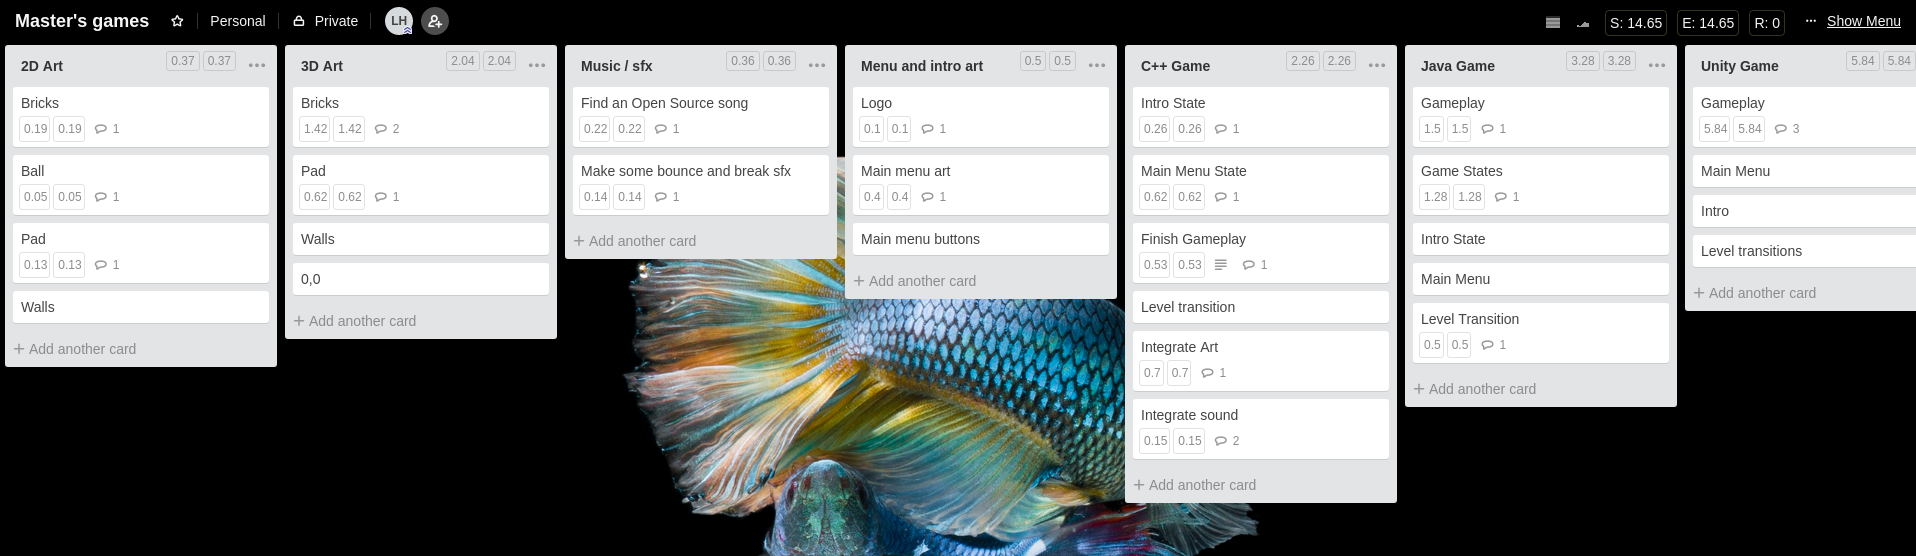
\includegraphics[width=14cm]{trelloBoardDemo}
	\caption{Primer table Trello.}.
	\label{slika:trelloDemo}
	\vspace*{-2em}
\end{figure}

HackNPlan je v osnovi podoben kot Trello, vendar je zgrajen specifično za razvoj računalniških iger. Poleg kanban table in organizacije ljudi ponuja še preglede statistik, vodenje sprintov ter funkcionalnost za skupno koncipiranje in dokumentiranje idej. Primer table vidimo na sliki \ref{slika:hacknplanDemo}. Vso našteto funkcionalnost dobimo v brezplačni verziji, ponujajo pa tudi nadgradnjo za dodatne storitve. Cena nadgradnje je 4 evre na mesec, glavna dodatna funkcionalnost pa so integracije z drugimi storitvami, kot so GitHub, Slack ipd. Brezplačnih integracij ni, zato je na tem področju slabši produkt kot Trello, vendar pa veliko pripomorejo specifične funkcionalnosti za namen razvoja iger.

\begin{figure}[h]
	\centering
	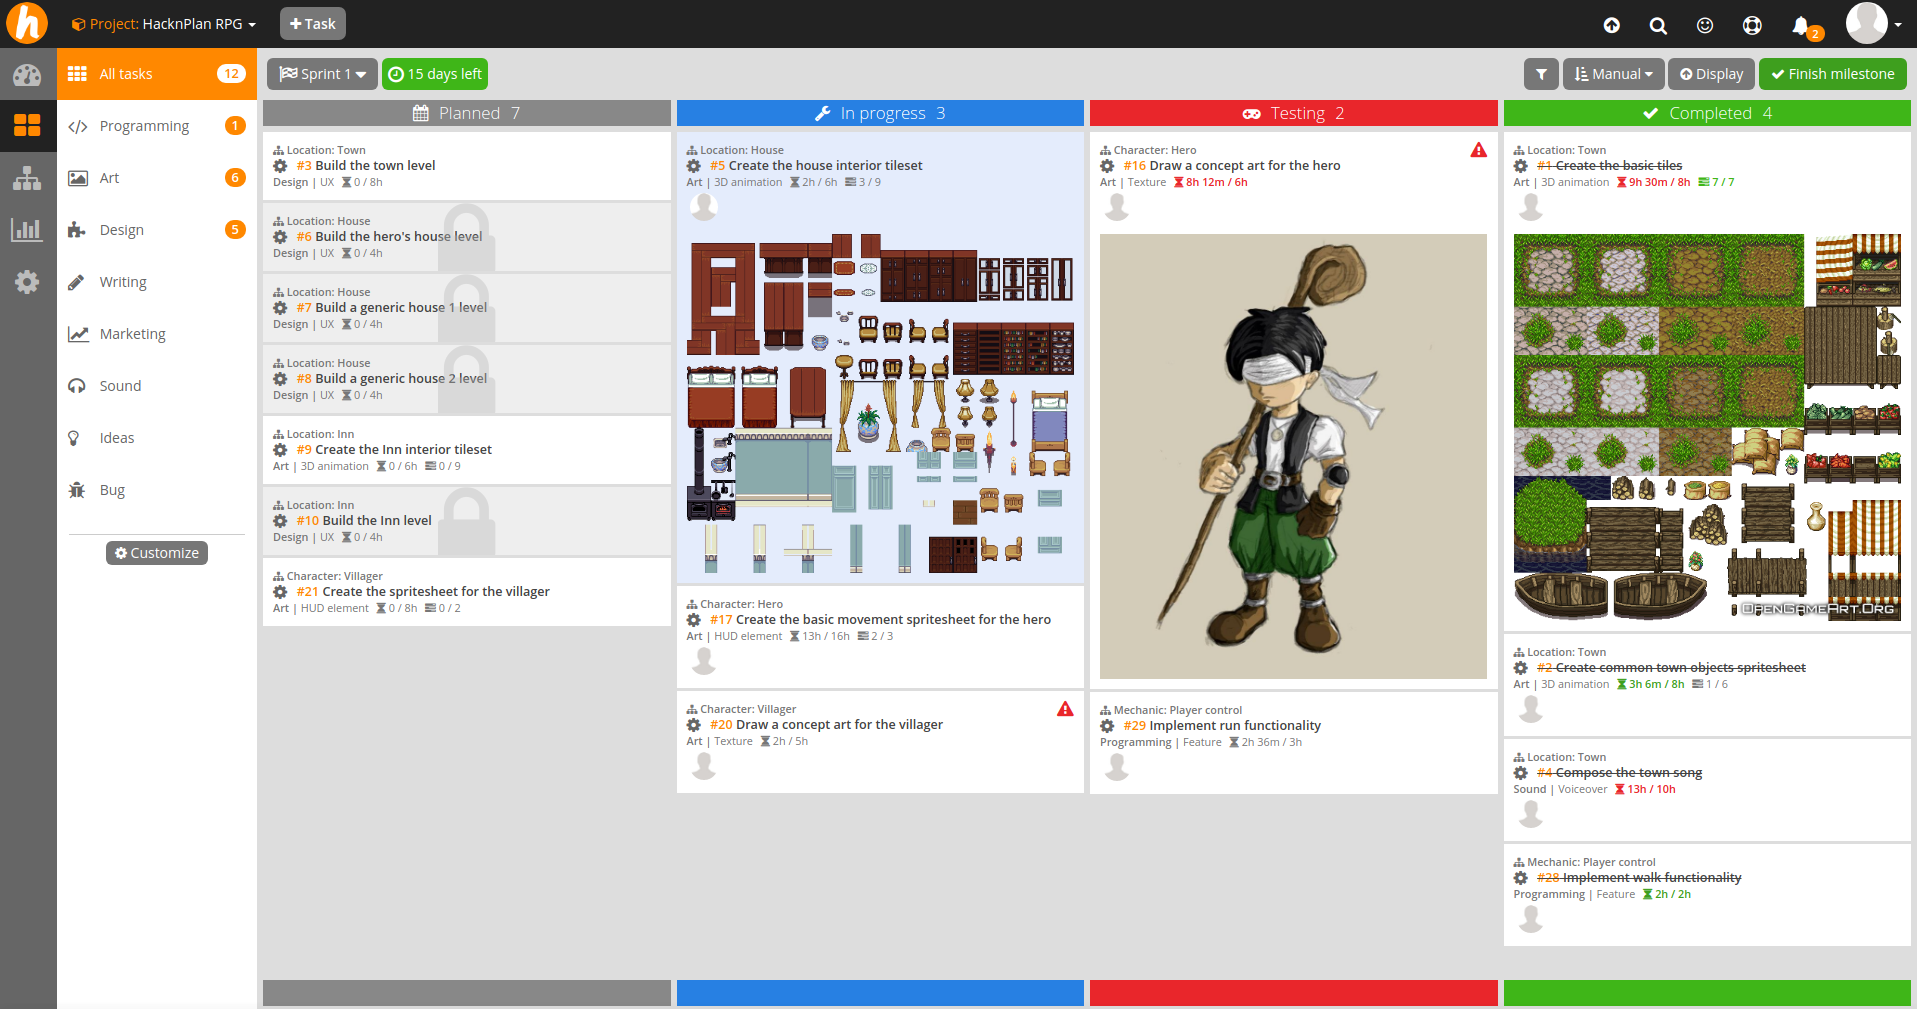
\includegraphics[width=13cm]{hacknplanDemo}
	\caption{Primer table HackNPlan.}.
	\label{slika:hacknplanDemo}
	\vspace*{-2em}
\end{figure}

\subsection{Organizacija projekta in kode}
Enako pomembna kot organizacija opravil je organizacija samega projekta med razvojem. Za te potrebe obstaja več rešitev verzioniranja projektov, kot so SVN, Mercurial, GIT, Perforce itd. Te programske rešitve ponujajo način hranjenja trenutnega stanja projektne kode na centralnem mestu, obenem pa sledijo vsem spremembam vsake datoteke. Možno je tudi hraniti več različnih aktualnih verzij iste datoteke v različnih vejah in jih nato združiti v končno obliko. Vsak razvijalec ima lokalno svojo kopijo projekta in svoje spremembe pošilja v centralni repozitorij. Tako v ozadju nastaja drevesna struktura sprememb projekta skozi čas. Primer takega grafa vidimo na sliki \ref{slika:gitGraph}. Vsaka sprememba je komentirana s strani razvijalca in tako je možno v primeru težav hitro poiskati in preiti na starejšo verzijo \cite{versionControl}.
	
\begin{figure}[h]
	\centering
	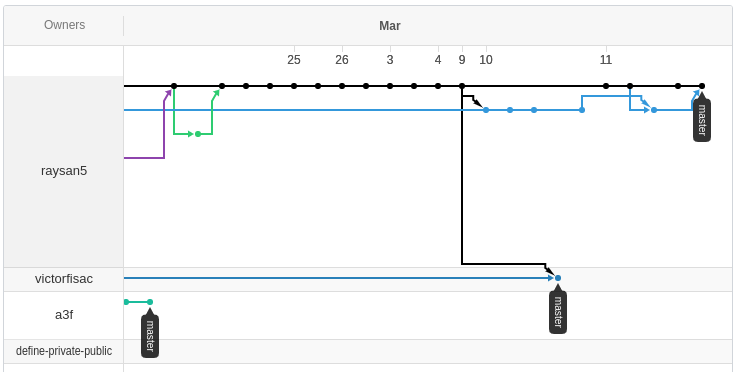
\includegraphics[width=13cm]{gitGraph}
	\caption{Primer grafa sprememb Raylib projekta na GitHub-u.}.
	\label{slika:gitGraph}
	\vspace*{-2em}
\end{figure}

V industriji razvoja računalniških iger je najbolj uporabljen sistem verzioniranja Perforce, saj deluje najboljše za večje projekte in kot komercialna plačljiva programska rešitve ponuja zelo močna orodja za delo z binarnimi datotekami (umetniški in zvočni gradniki so velikokrat v binarnem formatu in so obenem največje datoteke v projektu). Za večje projekte je Perforce plačljiv, ponujajo pa brezplačno različico za projekte do 5 ljudi.

Najbolj preprost za uporabo in najbolj razširjen pri razvoju programske opreme je sistem Git. Priljubljenost je v veliki meri povezana s storitvijo GitHub, ki ponuja oblačno hranjenje repozitorija z našim projektom, obenem pa nudi funkcionalnost za lažje skupno delo na projektu. Alternativa GitHub-u je BitBucket, obe rešitvi pa smo analizirali za potrebe razvoja igre.

GitHub je spletna platforma, zgrajena na bazi sistema verzioniranja Git. Glavna storitev je gostovanje našega repozitorija v oblaku, vendar imajo še obilo drugih storitev, zaradi česar so zelo priljubljeni za veliko projektov. Omogočajo upravljanje z ljudmi in skupinami, kdo ima dostop do kode, kdo dela na katerem opravilu ipd. Pregled sprememb je preprost za uporabo in omogoča komentiranje kode. Za vsak projekt nudijo tudi sistem sledenja napak (npr. kot Bugzilla), kjer lahko vsi, ki uporabljajo programsko opremo, javijo napake in komunicirajo z razvijalci. Zelo priljubljena funkcionalnost so tudi zahteve za spremembe (angl. \textit{pull request}), kjer lahko nekdo izdela in predlaga spremembe za projekt, nato pa se razvijalci odločijo, ali bodo te spremembe integrirali v glavno vejo projekta. Za odprtokodne in javne projekte je vsa ta funkcionalnost zelo dobrodošla, saj nudi lažje upravljanje s projektom. Brezplačna verzija Github-a ponuja vso našteto funkcionalnost, omejitev je le v tem, da morajo biti vsi naši projekti javni. Če hočemo imeti zasebni projekt na Github, je potrebno plačati 7 evrov mesečno \cite{github}.

Alternativa Github-u je storitev BitBucket. Ponuja enako funkcionalnost, vendar v brezplačni storitvi dovolijo zasebne repozitorije. Omejitev brezplačnega paketa je maksimalno 5 razvijalcev na projektu. Če hočemo povečati število razvijalcev, je cena 2 evra na razvijalca na mesec. Za projekte z manjšo skupino je torej BitBucket boljša rešitev za zasebni repozitorij. Če pa želimo, da je naš projekt na voljo vsem, pa je boljša alternativa GitHub \cite{bitBucket}.

\section{Orodja za izdelavo grafičnih gradnikov}
Grafični gradniki so pri razvoju računalniške igre uporabljeni od samega koncipiranja do končnega izida igre. Mi smo se osredotočili na gradnike, ki se uporabijo v sami računalniški igri. Ti gradniki so odvisno od tipa igre -- 2D slike ali 3D modeli. Na trgu obstaja veliko rešitev za izdelavo teh gradnikov, mi pa smo analizirali brezplačno programsko opremo, ki ima več kot dovolj funkcionalnosti za izdelavo gradnikov, potrebnih za individualne projekte.

\subsection{2D grafični gradniki}
Individualni projekti večinoma uporabljajo dva stila 2D grafičnih gradnikov: piksel umetnost (angl. \textit{pixel art}) in vektorska umetnost (angl. \textit{vector art}). Končni rezultat je kljub imenom vedno rastrska slika. Razlika je v tem, kako so gradniki ustvarjeni in kaj je v stilu pomembno. Piksel umetnost izhaja iz navdiha po starih igralnih sistemih, kjer so bile omejitve v smislu ločljivosti gradnikov in razpoložljivosti barv. Pomembno je izkoristiti vsak piksel, ki je na voljo. Nasprotno pa vektorski gradniki ciljajo na gradnike višje ločljivost. Uporabiti poskušajo preproste oblike in njihovo združevanje za pridobitev končnih slik. Razliko v stilih vidimo na sliki \ref{slika:pixelVsVector}.

\begin{figure}[h]
	\centering
	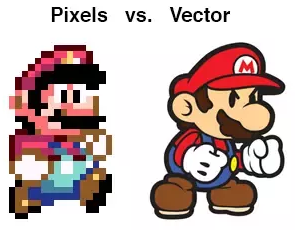
\includegraphics[width=6cm]{pixelVsVector}
	\caption{Razlika v stilih 2D grafičnih gradnikov. Vir \cite{pixelVsVector}}
	\label{slika:pixelVsVector}
\end{figure}

Program, ki ga priporočamo za izdelavo 2D piksel art gradnikov je Aseprite\footnote{https://www.aseprite.org/}. Vsa potrebna funkcionalnost za delo s slikami iz profesionalnih programov je na voljo, vendar so vse prilagojene za delo s slikami nižjih ločljivosti. Zelo močna so tudi orodja za delo z animacijami, plastmi ipd. Za namen razvoja računalniških iger nam ponuja tudi posebne izvoze v teksturne atlase in nize slik za animacijo. Program je na voljo za 15 evrov, vendar je vsa izvorna koda javna, zato si lahko uradno tudi sami zgradimo program in ga uporabljamo v komercialne namene. Prednost plačljive različice so samodejne posodobitve, ni potrebno prevajati izvorne kode ter seveda podpora nadaljnjega razvoja.

Za razvoj vektorske grafike pa predlagamo program Inkscape\footnote{https://inkscape.org/en/}. Po funkcionalnosti je podoben Adobe Illustratorju, le da je na voljo kot brezplačna odprtokodna rešitev. Manjkajo napredne funkcionalnosti kot je zvijanje združenih objektov za potrebe animacije, vendar na trgu ni boljše brezplačne alternative. V Inkscape delamo z vsemi liki kot z objekti in nad njimi lahko izvajamo booleanove transformacije (presek, unija, odštevanje ipd.) ter tako ustvarimo želene like. Ker delamo z objekti, je naš končni izdelek neodvisen od ločljivosti in ga lahko izvozimo v poljubni velikosti za našo igro. 

\subsection{3D grafični gradniki}
Izdelava 3D modelov je bolj zahtevna od 2D gradnikov, saj je potrebnih več korakov (modeliranje, teksture, animiranje). V industriji se uporabljajo različni programski paketi, kot so Maya, Houdini, ZBrush in Blender\footnote{https://www.blender.org/}. Od teh je Blender edini brezplačni in odprtokodni program, ki je na voljo na vseh operacijskih sistemih. V zadnjih letih je vedno bolj uporabljen v industriji, saj se s svojo funkcionalnostjo lahko kosa z drugimi plačljivimi programi in jih na določenih mestih celo preseže. Primer programa vidimo na sliki \ref{slika:blenderDemo}.

\begin{figure}[h]
	\centering
	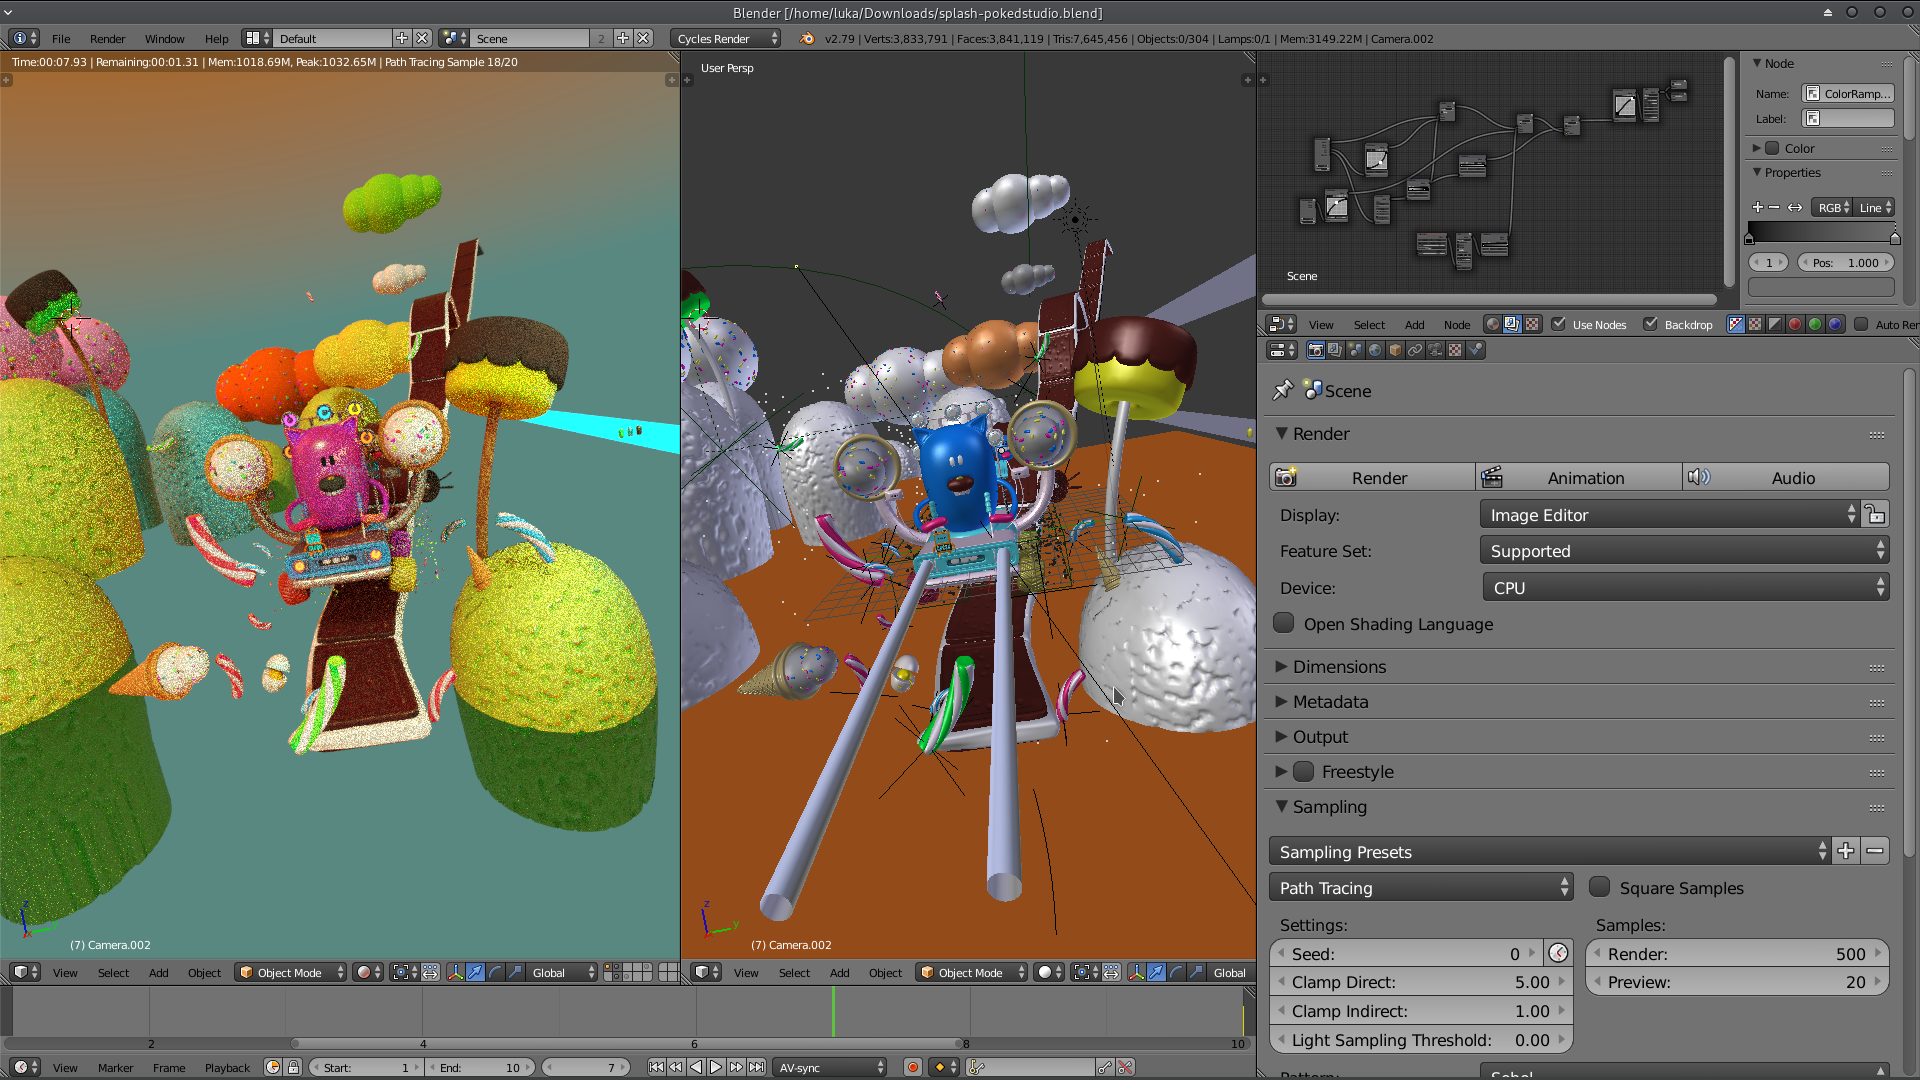
\includegraphics[width=13cm]{blenderDemo}
	\caption{Programski paket Blender}
	\label{slika:blenderDemo}
\end{figure}

\section{Orodja za izdelavo zvočnih gradnikov}
Za izdelavo zvočnih gradnikov (zvočnih efekti in glasba) smo podobno kot pri izdelavi grafičnih gradnikov analizirali brezplačne rešitve, ki ponujajo potrebne funkcionalnosti za razvoj. Glavna razlika med zvočnimi efekti in glasbo je, da se efekti uporabljajo za različne akcije v igri (npr. streli orožij, skok, šumenje ipd.), primerna glasba pa igra v ozadju glede na trenutno splošno dogajanje. Velikokrat se uporabljajo namenski programi za izdelavo glasbe tudi za izdelavo efektov, vendar obstaja nekaj orodij, ki so namenjene specifično za to.

Izdelava zvočnih efektov ima dva pristopa. Za bolj kakovostne efekte se v studiu posnamejo dejanski zvoki, ki bi bili primerni za igro. Recimo za strele orožij se posnamejo streli avtentičnih orožij, šumenje se simulira z listjem ipd. Ti zvoki se potem obdelajo in prilagodijo v programski opremi za delo z zvokom/glasbo. Drugi način je generiranje zvokov iz računalniško ustvarjenih zvokov in šumov. Z uporabo različnih valovnih oblik (sinusoida, trikotni val, rampa, kvadrat ipd.), filtrov in različnih modulacij ustvarimo želene efekte. Namenski programi za ta proces so Bfxr, Labchirp, DSP Retro/Anime ipd. Labchirp in DSP delujeta le na platformi Windows, obenem je DSP plačljiv, zato smo za analizo izbrali Bfxr\footnote{https://www.bfxr.net/}, ki je prosto dostopen in obenem uporaben kar s spleta. Program vidimo na sliki \ref{slika:bfxr}. Kot je razvidno s slike, imamo možnost izbire različnih valovnih funkcij, ki jih nato spreminjamo s ponujenimi drsniki. Ustvarjene efekte lahko tudi združimo skupaj in na koncu izvozimo v wav formatu za uporabo v igri.

\begin{figure}[h]
	\centering
	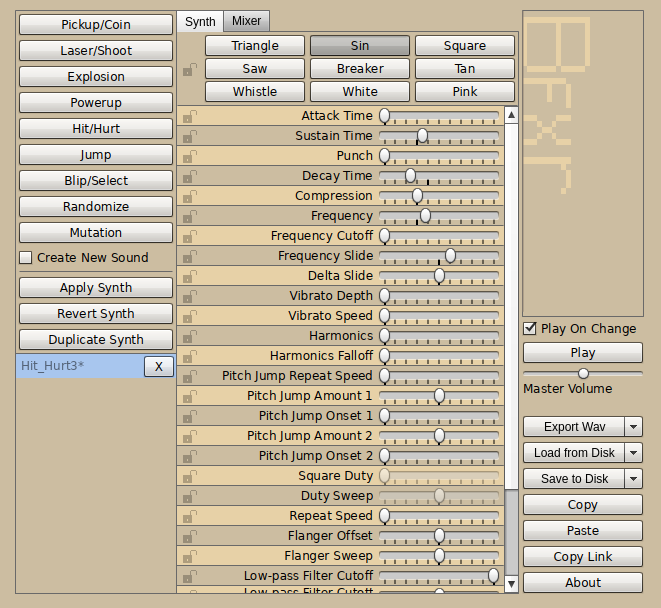
\includegraphics[width=10cm]{bfxr}
	\caption{Program Bfxr}
	\label{slika:bfxr}
\end{figure}

Izdelava glasbe je bolj pokrita s programskimi paketi kot izdelava efektov. Med bolj znane sodijo FL Studio, Reaper, Logic Pro X itd. Vsi našteti so plačljivi z minimalno vstopno ceno vsaj 100 evrov. Obstaja tudi nekaj prosto dostopnih rešitev, kot so Ardour in LMMS\footnote{https://lmms.io/}, ki smo ga bolj podrobno analizirali. Je odprtokodni program in je na voljo na vseh operacijskih sistemih (Windows, Linux, OS X). Na sliki \ref{slika:lmms} vidimo primer izdelave skladbe. Izberemo si različne inštrumente (na voljo so godala, tolkala, pihala, klaviature, možno si je tudi ustvariti sintetično glasbilo) in z njimi ustvarimo vse potrebne dele skladbe s postavljanjem posameznih not. S tem ustvarimo sekcije, ki jih nato sestavljamo v končni produkt.

\begin{figure}[h]
	\centering
	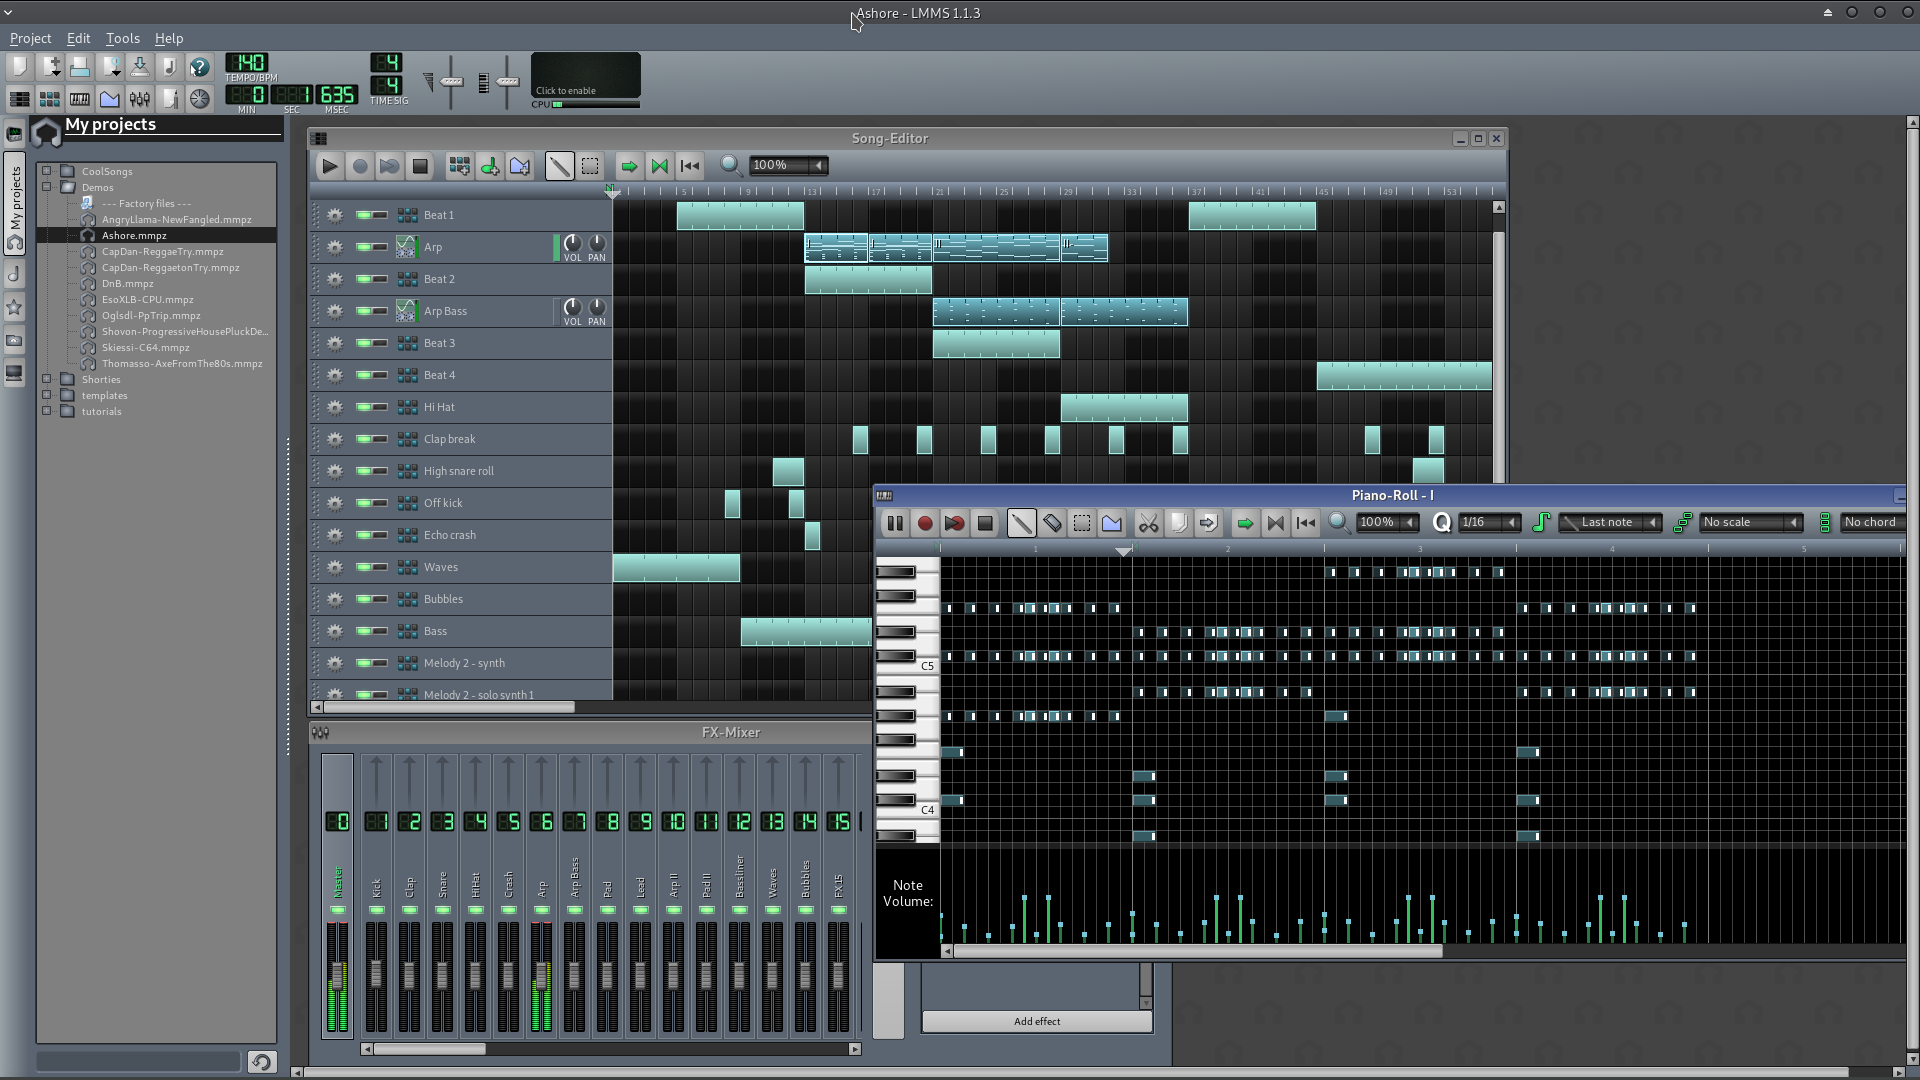
\includegraphics[width=12cm]{lmms}
	\caption{Program LMMS med izdelavo skladbe}
	\label{slika:lmms}
\end{figure}

\section{Računalniške knjižnice, ogrodja in pogoni}
Glavni cilj magistrskega dela je uporabiti in opisati orodja za tehnično implementacijo računalniške igre. S tehnično implementacijo mislimo samo programiranje oziroma razvoj igre. Zato smo v tem poglavju raziskali in opisali različna orodja, njihova uporaba in prakse pa sledijo v poglavju \ref{chapter:razvojIger}. Omejili smo se na orodja, ki so na voljo na vseh večjih operacijskih sistemih (Windows, Linux in OS X) in je z njimi možno izdelati računalniško igro za vse tri sisteme (po možnosti tudi več kot npr. mobilne in spletne platforme).

Tehnično implementacijo računalniške igre smo v našem delu kategorizirali v tri različne smernice: nizkonivojske knjižnice, visokonivojske knjižnice, ogrodja ter namenske pogone.

\subsection{Nizkonivojske knjižnice}
V to kategorijo smo uvrstili knjižnice, ki nudijo specifičen nabor funkcionalnosti, potrebnih za razvoj računalniške igre. Omejili smo se na programski jezik C++, saj je najbolj razširjen v industriji razvoja iger. Te knjižnice pokrivajo eno ali več izmed naslednjih funkcionalnosti: upravljanja z okni, vhodni sistemi (tipkovnica, miška, igralni ploščki ipd.), računalniška grafika, predvajanje zvoka, medmrežna komunikacija, matematične funkcije, fizikalni pogoni itd. Težko je definirati mejo med knjižnico in ogrodjem (angl. \textit{framework}), vendar v splošnem knjižnice v tej kategoriji ne pokrivajo vseh potrebni funkcionalnosti za razvoj. Potrebno je uporabiti njihovo kombinacijo, da uresničimo končni projekt.

Najprej je potrebna osnovna knjižnica, ki ponuja funkcionalnost za vzpostavitev programa. Sem spadata knjižnici SDL\footnote{https://www.libsdl.org/}\cite{sdllib} in GLFW\footnote{http://www.glfw.org/}\cite{glfw}. Obe ponujata abstrakcijo za potrebno delo z okni na namizju, dostop do vhodnih naprav, kontekst za upravljanje z grafičnim cevovodom, kot je OpenGL, Direct3D ali Vulkan ipd. Sta temelj večini iger, ki se razvijajo z nizkonivojskimi knjižnicami, obenem pa sta tudi izhodiščna točka za namenske pogone, kot je Source Engine \cite{sourceEngineSDL} in Cryengine \cite{cryengineSDL}.

Preden nadaljujemo, je potrebno omeniti še grafične cevovode. Tukaj obstajajo trenutno trije standardi: Direct3D, OpenGL in Vulkan. Direct3D je član paketa DirectX, skupka knjižnic za razvoj računalniških iger od podjetja Microsoft. Podobno kot SDL ponuja DirectX paket vseh potrebnih funkcionalnosti za razvoj, vendar je na voljo samo za Windows platformo in igralno konzolo Xbox. Zato nismo opisali grafičnega cevovoda Direct3D, saj ni na voljo za vse platforme. OpenGL in Vulkan pa sta standarda za delo z grafičnim cevovodom, razvoj nad njima vodi konzorcij Khronos Group. OpenGL so začeli razvijati leta 1992, Vulkan pa je naslednik tega standarda in se je pričel razvijati leta 2016. Oba standarda ponujata način dela z grafičnimi karticami za potrebe izrisovanja 2D in 3D grafike. Oba standarda imata svoje knjižnice, ki za delo potrebujejo samo kontekst do grafične kartice, ki ga ponudi osnovna knjižnica kot je SDL ali GLFW \cite{opengl}. 

SDL ponuja še razširitve v obliki dodatnih knjižnic za dostop do specifične funkcionalnosti:
\begin{itemize}
	\item \textbf{SDL\_Image}. SDL v osnovi ponuja podporo za omejeno število slikovnih formatov. Pri branju drugih formatov potrebujemo dodatno knjižnico. SDL\_Image ponuja podporo za priljubljene formate BMP, GIF, JPEG, PNG, SVG ipd. Obenem so funkcije pripravljene tako, da je lažje uporabljati te slike v kontekstu knjižnice SDL, kot če bi uporabljali katero bolj splošno knjižnico za slike kot je SOIL \cite{sdlimage}.
	\item \textbf{SDL\_Mixer}. Osnovna knjižnica SDL podpira nalaganje glasbenih datotek v formatu wav. Obenem je možno predvajati zvoke po samo enem kanalu naenkrat, kar pomeni, da ne moremo predvajati več različnih efektov naenkrat, brez da bi sami spisali algoritem za mešanje efektov. Zato ponujajo razširitveno knjižnico SDL\_Mixer, ki odpravi te omejitve. Doda tudi podporo za branje datotek formata FLAC, OGG, MP3, MOD in MIDI. Obenem ponuja prevajanje zvokov po več različnih kanalih. Tako lahko predvajamo glasbo v ozadju, v ospredju pa predvajamo več različnih zvočnih efektov naenkrat \cite{sdlmixer}.
	\item \textbf{SDL\_TTF}. SDL ne podpira dela z računalniškimi pisavami (angl. \textit{font}). Če hočemo tekst izpisovati na zaslonu, moramo narediti slike črk in potem sestaviti besedilo iz posameznih slik. Tak postopek je zakompliciran in časovno potraten, obenem je za prehod med različnimi stili pisav potrebno znova ustvariti slike črk. SDL\_TTF doda podporo za branje standardnega formata računalniških pisav TTF. Tako lahko enostavno izpišemo besedila v poljubnem stilu na zaslon \cite{sdlttf}.
	\item \textbf{SDL\_Net}. Osnovna knjižnica ne ponuja nobene funkcionalnosti za komunikacijo preko mreže. SDL\_Net nam ponuja funkcionalnost za vzpostavitev strežnika in povezave na druge strežnike preko protokola TCP ali UDP. Razširitev deluje med različnimi platformami, tako da ni potrebno programirati specifične funkcionalnosti za vsako posebej \cite{sdlnet}.
	\item \textbf{SDL\_Rtf}. Ta razširitev ni najbolj uporabna za namene izdelave iger, ampak ker je še zadnja od uradno ponujenih, smo jo vseeno omenili. Ponuja funkcionalnost za delo z datotekami RTF. To so tekstovne datoteke z obogateno vsebino. Omogoča nam prikaz obogatene vsebine v naši aplikaciji SDL.
\end{itemize}

Seveda ni potrebno, da uporabljamo razširitve SDL, če uporabljamo SDL kot osnovo za našo igro. Razširitve ponujajo osnovno pomoč za delo s specifično funkcionalnostjo (zvok, računalniško besedilo, slike ipd.), vendar pa velikokrat nimajo naprednih funkcionalnosti, ki bi jih potrebovali za našo igro. Obenem razširitev ne moremo uporabljati, če za osnovo vzamemo knjižnico kot je GLFW. Zato smo opisali še nekaj izbranih drugih knjižnic, ki ponujajo večji nabor funkcionalnosti za razvoj igre:
\begin{enumerate}
	\item \textbf{SOIL} je kratica za \textit{Simple OpenGL Image Library}. Kot je že iz imena razvidno, nam ponuja branje slik za uporabo v naši aplikaciji. Podpira podobno funkcionalnost kot SDL\_Image, vendar je izdelana specifično za uporabo z OpenGL cevovodom, saj nam prebere slike v teksture za lažjo uporabo \cite{soil}.
	\item \textbf{Irrklang}. Ponuja napredno funkcionalnost za delo z zvokom. Osnovna funkcionalnost (podobno kot pri SDL\_Mixer) je nadgrajena s podporo za 3D zvok, s katerim se lahko v naši igri igralci orientirajo. Prav tako ponuja večji nabor efektov, ki jih lahko apliciramo na naših zvokih (npr. odmev, distorzija ipd.). Knjižnica je na voljo brezplačno, če delamo na nekomercialnem produktu, sicer pa moramo plačati enkratno licenco v višini 65 evrov (za uporabo v igrah, ki stanejo manj kot 20 evrov), 290 evrov (za igre do 27 evrov) oziroma licenco za specifično igro (brez omejitve cene) v višini 490 evrov \cite{irrklang}. 
	\item \textbf{FMOD}. Je ena izmed bolj priljubljenih zvočnih knjižnic za uporabo v razvoju iger. Ponujajo vso funkcionalnost od SDL\_Mixer in Irrklang, obenem pa ponujajo svojo platformo za nakupovanje zvočnih efektov in njihovo urejanje. Knjižnica je na voljo brezplačno za eno igro na leto, če je naš proračun manjši od 500 tisoč dolarjev. Za večje projekte pa stane licenca 5000 dolarjev \cite{fmod}.
	\item \textbf{FreeType}. Je osnovna knjižnica, na kateri je zgrajen SDL\_TTF. Če ne uporabljamo SDL knjižnice, potem moramo namesto razširitve uporabiti FreeType knjižnico. Ponuja enako funkcionalnost, kot smo že opisali pri SDL\_TTF, saj je tisto le ovoj za lažje delo s FreeType knjižnico v SDL aplikaciji \cite{freetype}.
	\item \textbf{Box2D in ReactPhysics3D}. Nizkonivojske osnovne knjižnice za razvoj iger po navadi nimajo podpore za delo z fizikalnim pogonom. Če hočemo simulirati interakcijo objektov kot v resničnem svetu, potem fizikalni pogon potrebujemo. Box2D je eden izmed najbolj priljubljenih za 2D igre in ponuja funkcionalnost za preverjanje trkov med različnimi objekti (podpira konkavne in konveksne oblike, visoke hitrosti, hitro iskanje pri visokem številu objektov) in svoj fizikalni pogon. Sam pogon podpira realno časovno simulacijo teles, upora, trenja, navorov, delo z zgibi, odzivi na sile ipd. Podobno funkcionalnost vendar v 3D prostoru ponuja knjižnica ReactPhysics3D. Obe knjižnici sta odprtokodni in na voljo brez licence \cite{box2d} \cite{reactPhysics3d}.
\end{enumerate}

\subsection{Visokonivojske knjižnice in ogrodja}
Težko je določiti mejo med nizkonivojskimi in visokonivojskimi knjižnicami oziroma ogrodji. V osnovi naj bi visokonivojske ponujale kompletno funkcionalnost, ki jo potrebujemo za razvoj igre od začetka do konca. Mogoče je kdaj potrebno dodati še knjižnico za zelo specifično funkcionalnost. Obenem take knjižnice priporočajo oziroma se naslanjajo na specifičen način razvoja igre, čemur se moramo prilagoditi, da najbolje izkoristimo funkcionalnost. 

Najprej smo v tem poglavju opisali še dve knjižnici, ki nista še popolnoma v tej kategoriji visokonivojskih knjižnic, vendar ponujata dovolj velik sklop funkcionalnosti, da ju ne moremo uvrstiti v našo definicijo čiste nizkonivojske knjižnice:
\begin{enumerate}
	\begin{figure}[h]
		\centering
		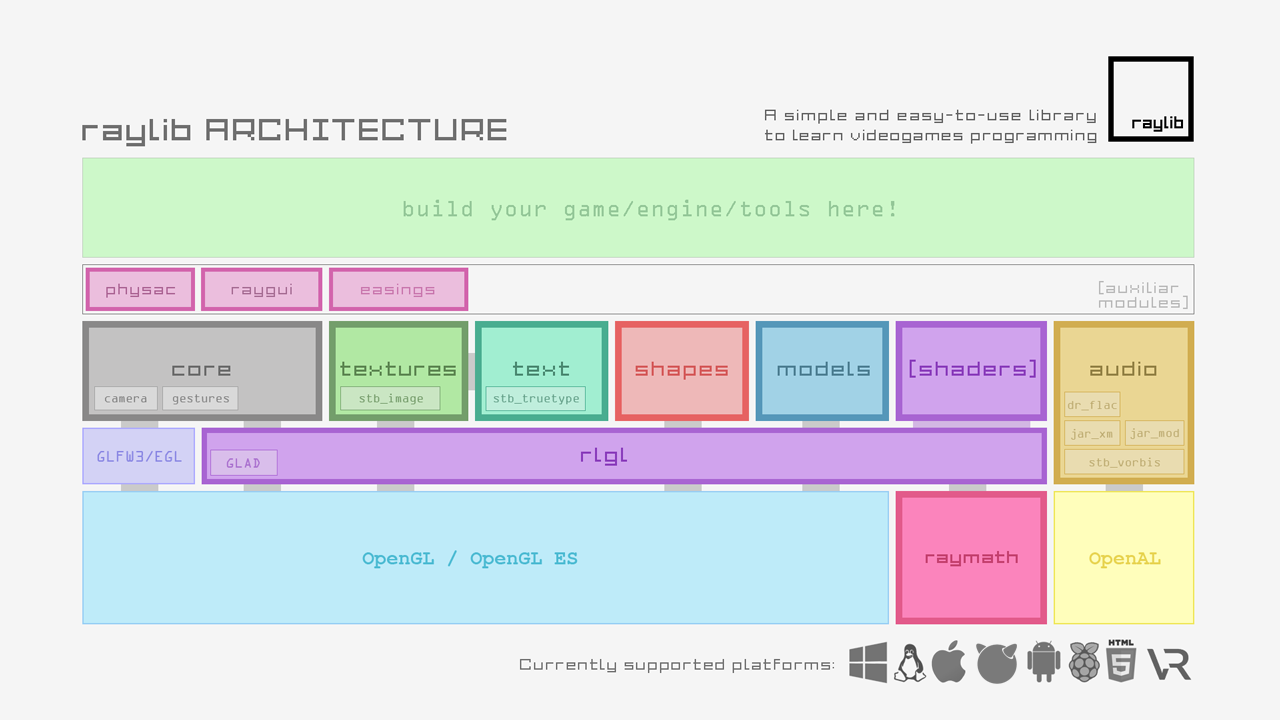
\includegraphics[width=12cm]{raylib_architecture}
		\caption{Arhitektura knjižnice Raylib. Vir \cite{raylib}}
		\label{slika:raylib}
	\end{figure}
	\item \textbf{Raylib}. Je odprtokodna C knjižnica, ki ponuja večji del funkcionalnosti za razvoj računalniške igre. Zgrajena je na osnovi GLFW in ima svoj sistem za delanje z okni ter vhodnimi napravami. Podpira branje in risanje slik različnih formatov, branje in risanje računalniških pisav, nalaganje 3D modelov in izrisovanje, sistem za materiale za modele, podporo senčilnikov (angl. \textit{shader}), predvajanje glasbe in zvokov, VR izrisovanje ipd. Knjižnica je nekako kombinacija vseh SDL knjižnic, vendar z nadgrajeno funkcionalnostjo. Ena večjih funkcionalnosti, ki manjka, je komunikacija preko mreže. Ponuja še dodatne individualne knjižnice, ki dodajo funkcionalnost za delo s preprostimi grafičnimi vmesniki, fizikalnim pogonom in animacijami. Te dodatne razširitvene knjižnice ne ponujajo kompletne funkcionalnosti, ki bi jih dobili z drugimi knjižnicami, zato nam tukaj manjka določen del funkcionalnosti. Knjižnica je zamišljena na način, da ne predvideva specifičnega načina programiranja, zato jo lahko uporabimo na svoj način \cite{raylib}. Arhitekturo knjižnice vidimo na sliki \ref{slika:raylib}.
	\item \textbf{SFML}. SFML je odprtokodna C++ knjižnica, ki ponuja bolj omejen sklop funkcionalnosti kot Raylib. Ima svojo zasnovo za delo s platformo in ne uporablja SDL ali GLFW. Podpira bolj osnovne funkcionalnosti, kot je izrisovanje, delanje z zvokom, vhodnimi napravami, računalniškimi pisavami, slikami in komunikacijo preko mreže. Nima napredne funkcionalnosti kot 3D izrisovanje, materiale, senčilnike ipd. Obenem ne ponuja nobenih razširitvenih knjižnic, s katerimi bi lahko dodali tako funkcionalnost \cite{sfml}. 
\end{enumerate}

Sledijo ogrodja, ki sodijo v kategorijo visokonivojskih knjižnic in ogrodij. To so ogrodja, ki so zgrajena z namenom izdelave računalniških iger in tako ponujajo vso funkcionalnost, ki bi jo rabili. Imajo svoj način uporabe, vendar nam s tem olajšajo delo, ki je potrebno za uresničitev naših ciljev.

LibGDX je ogrodje za programski jezik Java. Je odprtokodno in podpira vse namizne platforme, kot tudi Android, iOS ter izvajanje v brskalnikih. Ima zelo močan pogon za izrisovanje 2D in 3D grafike, obenem pa ponuja dostop do nizkonivojskih funkcij, če jih rabimo. Izrisovanje različnih objektov se zapakira skupaj, kar doprinese k hitrosti ogrodja. Podpira več vrst glasbenih in slikovnih formatov, delo z vhodnimi napravami ter gestami, ima obsežno funkcionalnost za matematične operacije, podpira 2D in 3D fizikalni pogon, mrežno komunikacijo, razna dodatna orodja in še veliko več. Skoraj vsa potrebna funkcionalnost, da izdelamo igro od začetka do konca, je v tem ogrodju. Ponuja scenski sistem za delo z našimi objekti v igri, kar nakazuje na specifičen način izdelovanja naše igre s pomočjo scen. Ni pa ta funkcionalnost obvezna \cite{libgdx}.

Monogame je ogrodje za programski jezik C\#. Ogrodje je nastalo kot nadomestek Microsoftovega XNA ogrodja, ko je Microsoft prekinil podporo za XNA, in je kompatibilno s kodo, ki je bila spisana za obstoječo knjižnico. Dandanes se je Monogame skupaj z Mono ogrodjem razvil v kompletno rešitev za izdelavo računalniških iger. Podpira podoben nabor funkcionalnosti kot LibGDX, z izjemo manjkajočega fizikalnega pogona. Tega lahko vključimo na primer z uporabo Box2D ipd. Monogame je odprtokoden in na voljo za vse večje platforme \cite{monogame}.

Cocos2D je zbirka različnih ogrodij za razvoj iger. Začetek razvoja je bilo ogrodje za programski jezik Python, nakar se je projekt odcepil v več ogrodij. Dandanes so v Cocos2D družini sledeča ogrodja: Cocos2D (originalno ogrodje za Python), Cocos2D-Swift (za programski jezik Swift in iOS platformo), Cocos2D-XNA (podobno kot projekt Monogame, je ta različica izdelana kot nadgradnja XNA ogrodja, danes pa deluje na Monogame), Cocos2D-JS (za programski jezik JavaScript ter razvoj računalniških iger za spletni brskalnik) in Cocos2D-X (največje ogrodje v tej družini, za programski jezik C++). Najbolj priljubljena veja ogrodja je Cocos2D-x, ki je tudi najbolj vzdrževana. Je odprtokodna in deluje na vseh večjih platformah. Ima zelo podoben nabor funkcionalnosti kot LibGDX in Monogame ter vključuje tudi fizikalni pogon Box2D in Chimpmunk. Razvijalci Cocos2D družine pa ponujajo tudi Cocos Studio, ki deluje kot namenski pogon za razvoj iger in temelji na Cocos2D-X ogrodju. Vsa ogrodja iz te družine temeljijo na delu s Sprite-i. Vsa logika se vrti okoli teh objektov, zato se moramo temu prilagoditi za produktivno delo v tem ogrodju \cite{cocos2d}\cite{cocos2dx}.

\subsection{Namenski pogoni}
Namenski pogoni so višek današnje tehnologije za razvoj računalniških iger. Na trgu obstaja več različnih pogonov, vendar daleč pred vsemi vodita razvoj Unity od Unity Technologies in Unreal Engine od podjetja Epic. Oba nudita svoj urejevalnik, v katerem grafično izdelujemo računalniško igro in tako pohitrimo razvoj, na voljo pa nam je vsa funkcionalnost, ki bi jo potrebovali za kompletni razvoj iger. Vsak ima tudi svojo trgovino, v kateri lahko kupimo gradnike za igro ter dodatne funkcionalne razširitve za potrebe razvoja. Sta nekako zaprt ekosistem, v katerem razvijamo vse.

Unity je prvič izšel leta 2005. Pogon je zgrajen v programskem jeziku C++, razvijalcem pa ponuja vmesnik za namensko programiranje v C\#. Ponuja vso funkcionalnost, ki smo jo našteli v drugih knjižnicah in ogrodjih doslej ter še veliko več. Pogon uporabljajo profesionalni studii po vsem svetu za razvoj iger in je najbolj priljubljen za individualne razvijalce med namenskimi pogoni. Glavne prednosti pred drugimi pogoni so preprosta uporaba, nizka stopnja potrebnega znanja, ogromen nabor dokumentacije in vodičev za izdelavo iger, hitro iskanje odgovorov (zaradi priljubljenosti hitro najdemo rešitev na našo težavo) ter velik nabor dodatne funkcionalnosti preko Unity trgovine kar iz orodja za razvijanje. Med funkcionalnostmi za razvoj ponuja tudi enostavno vgradnjo sistema za nakupovanje v naši igri ter oglase. Ponujajo tudi oglaševanje naše aplikacije skozi vse druge igre, ki uporabljajo Unity oglase in tako hitro dosežemo nove igralce. Za razvoj iger za več igralcev preko spleta imajo strežnike in integracijo kar preko Unity Editor-ja.

V preteklosti je bila določena funkcionalnost nedostopna brezplačnim uporabnikom, dandanes pa omejitev več ni. Edina omejitev pri brezplačni verziji je, da moramo pri zagonu naše igre obvezno prikazati Unity logotip ter da so namenski strežniki za našo igro omejeni na 20 igralcev naenkrat. Brezplačna verzija nam je na voljo, če naše podjetje na leto zasluži manj kot sto tisoč dolarjev. Za prihodke od sto tisoč do dvesto tisoč potrebujemo Unity Plus licenco za 35 dolarjev mesečno, za večje prihodke pa potrebujemo Unity Pro licenco, ki stane 125 dolarjev mesečno. Plačljive licence dovolijo, da ne prikažemo Unity logotipa na začetku igre, več igralcev istočasno na njihovem strežniku, dodatno analizo za izdano igro, direktno podporo od Unity razvijalcev, 20-odstotni popust na vse izdelke iz Unity trgovine in še več. Unity Technologies ponujajo tudi alternativo sistema za verzioniranje, ki nam omogoča lažjo sinhronizacijo med drugimi sodelavci in je vgrajen v Unity Editor \cite{unityFeatures}.

Unreal Engine ima daljšo zgodovino kot Unity -- prvotna verzija pogona je izšla leta 1998. Prva in druga verzija nista bili na voljo za prosto uporabo, tretja verzija pa je pripeljala SDK za širšo uporabo. Četrta verzija pogona leta 2014 je zaznamovala začetek dostopnega in odprtokodnega namenskega pogona, ki ga je lahko uporabljal vsak. Pogon je razvit v jeziku C++ in ponuja razvijalcem namenski programski vmesnik. Funkcionalnost je podobna Unity Engine-u, vendar je večji poudarek na tehnološkem napredku in naprednih grafičnih izrisovanjih. Pogon je bolj priljubljen pri večjih profesionalnih studiih, ki hočejo izrabiti napredno funkcionalnost pogona. Glavne prednosti pred drugimi pogoni so prosto dostopna izvorna koda, večji in bolj tehnološko dovršen nabor funkcionalnosti, možnost vizualnega programiranja ter bolj dodelano in performantno jedro pogona. Licenciranje je drugačno od Unity-ja, uporaba je brezplačna brez omejitev, ko pa igro izdamo, pa moramo podjetju Epic plačati 5 \% vseh prihodkov igre \cite{unrealEngine}. 

Odločitev med pogonoma je odvisno od naših potreb za projekt. Unity licenciranje in lažja dostopnost je prednost pri manjših projektih, kjer ne potrebujemo najnovejših funkcionalnosti za razvoj. Pri profesionalnih projektih začneta izstopati dve največji pomanjkljivosti pogona Unity . Prva je specifične manjkajoče funkcionalnosti, ki jih moramo nato za dodaten denar kupiti na Unity trgovini in so mogoče že privzeto vključene v Unreal Engine (Unreal Engine je bolj celovit paket pogona, kjer nam ni potrebno dodatnih funkcionalnosti doplačevati, kar je velika prednost). Druga pomanjkljivost pogona Unity  pa je slabša grafična podoba, kot jo doseže Unreal Engine. Unity Technologies si trenutno zadaja cilj, da ti dve pomanjkljivosti odpravi, vendar je trenutno za bolj kompleksne projekte priporočljiv Unreal Engine. Po drugi strani pa je prednost Unity-ja pred Unreal Engine boljša mobilna podpora in nižja potrebna strojna zmogljivost za igranje igre. Nižja potrebna računalniška moč je preferenčna pri manjših ali individualnih projektih. Kakor koli že, za vsak projekt moramo individualno oceniti, kaj potrebujemo in kateri pogon bolj ustreza našim potrebam.
	
\chapter{Razvoj računalniške igre}\thispagestyle{fancy}
\label{chapter:razvojIger}
V tem poglavju smo se posvetili metodam in praksam, ki smo jih uporabili pri razvoju računalniške igre. Metode smo kategorizirali glede na namen uporabe in opisali možnosti uporabe v orodjih RayLib, LibGDX in Unity.
\section{Uporabljena orodja}
V sklopu magistrskega dela smo se odločili, da izdelamo računalniško igro v treh različnih orodjih za razvoj iger:
\begin{itemize}
	\item Knjižnica RayLib v programskem jeziku C++. Kot omenjeno je RayLib prehodna knjižnica med nizkonivojskimi in visokonivojskimi knjižnicami. Ima vso glavno funkcionalnost, potrebno za razvoj, vendar ji manjka olajševalna funkcionalnost, ki smo jo morali sami razviti. Tako je najbolj primerna za razvoj igre iz nizkonivojskega zornega kota.
	\item Ogrodje LibGDX v programskem jeziku Java. Je eno izmed najbolj funkcionalno polnih ogrodij, ki še ni samo za sebe namenski pogon s svojim načinom dela, zato je odlično za prikaz razvoja, kjer se ne podrejamo načinu dela z pogonom.
	\item Namenski pogon Unity. Najbolj priljubljen namenski pogon za razvoj iger je potrebno skoraj obvezno vključiti v primerjavo. Nudi ogromno funkcionalnosti, nizko vstopno težavnost in preprostost za uporabo. Z Unity smo lahko prikazali enostavnost razvoja iger.
\end{itemize}

Poleg zgoraj omenjenih orodij smo potrebovali še orodja za izdelavo grafičnih in zvočnih gradnikov. Za izdelavo 2D gradnikov smo uporabili vektorsko orodje Inkscape ter izvozili slike v rastrski format. Za izdelavo 3D modelov smo uporabili Blender, saj kot že omenjeno nudi vso potrebno funkcionalnost. Za izdelavo zvočnih efektov smo se poslužili orodja Bfxr ter zvoke pretvorili v ustrezni format z orodjem Audacity.

Med samim razvojem smo si razgradili delo na platformi Trello, ves napredek pa smo verzionirali s sistemom Git ter naš repozitorij hranili na platformi GitHub. Vsa vsebina, izdelana za potrebe magistrskega dela (koda, gradniki, projekti in magistrsko delo v Latex formatu), je na voljo na sledeči povezavi: \url{https://github.com/cimpresovec/Masters}. Vsebina uporablja MIT licenco, kar pomeni, da je prosto dostopna za uporabo brez omejitev.

\section{Igra Breakout}
Računalniška igra, ki smo jo izdelali v sklopu magistrskega dela je klon igre Breakout. Cilj izdelave je bila tehnična izvedba, saj smo z implementacijo klona preskočili fazo načrtovanja. Originalna igra je izšla leta 1976 za Atari, vendar je do danes izšlo na desetine variacij igre. V igri igralec nadzira lopar, s katerim odbija žogo v omejenem prostoru. Lopar je omejen na spodnji del zaslona in se lahko premika samo horizontalno. Z odbijanjem žoge poskuša igralec uničiti vse ovire v stopnji, od katerih se žoga odbija, ko jih uničuje. Cilj je čim bolj spretno odbijati žogo, nabrati čim več pik ter napredovati skozi stopnje z uničenjem vseh ovir. Če se žoga igralcu izmuzne, izgubi eno življenje ter lahko poskusi znova. Odbijanje žoge od loparja je prilagojeno tako, da ima igralec visoko stopnjo nadzora nad tem, v katero smer se bo odbila žoga.

Vse verzije igre (C++, Java in Unity) so zaključene celote in vsebujejo naslednje glavne funkcionalnosti:
\begin{itemize}
\item Naslovni zaslon, kjer prikažemo naš logotip igre. Pri namenskem pogonu Unity smo morali prikazati še Unity logotip, saj smo uporabljali brezplačno verzijo orodja. Zaslon lahko vidimo na sliki \ref{slika:naslovniZaslon}.
\begin{figure}[h]
	\centering
	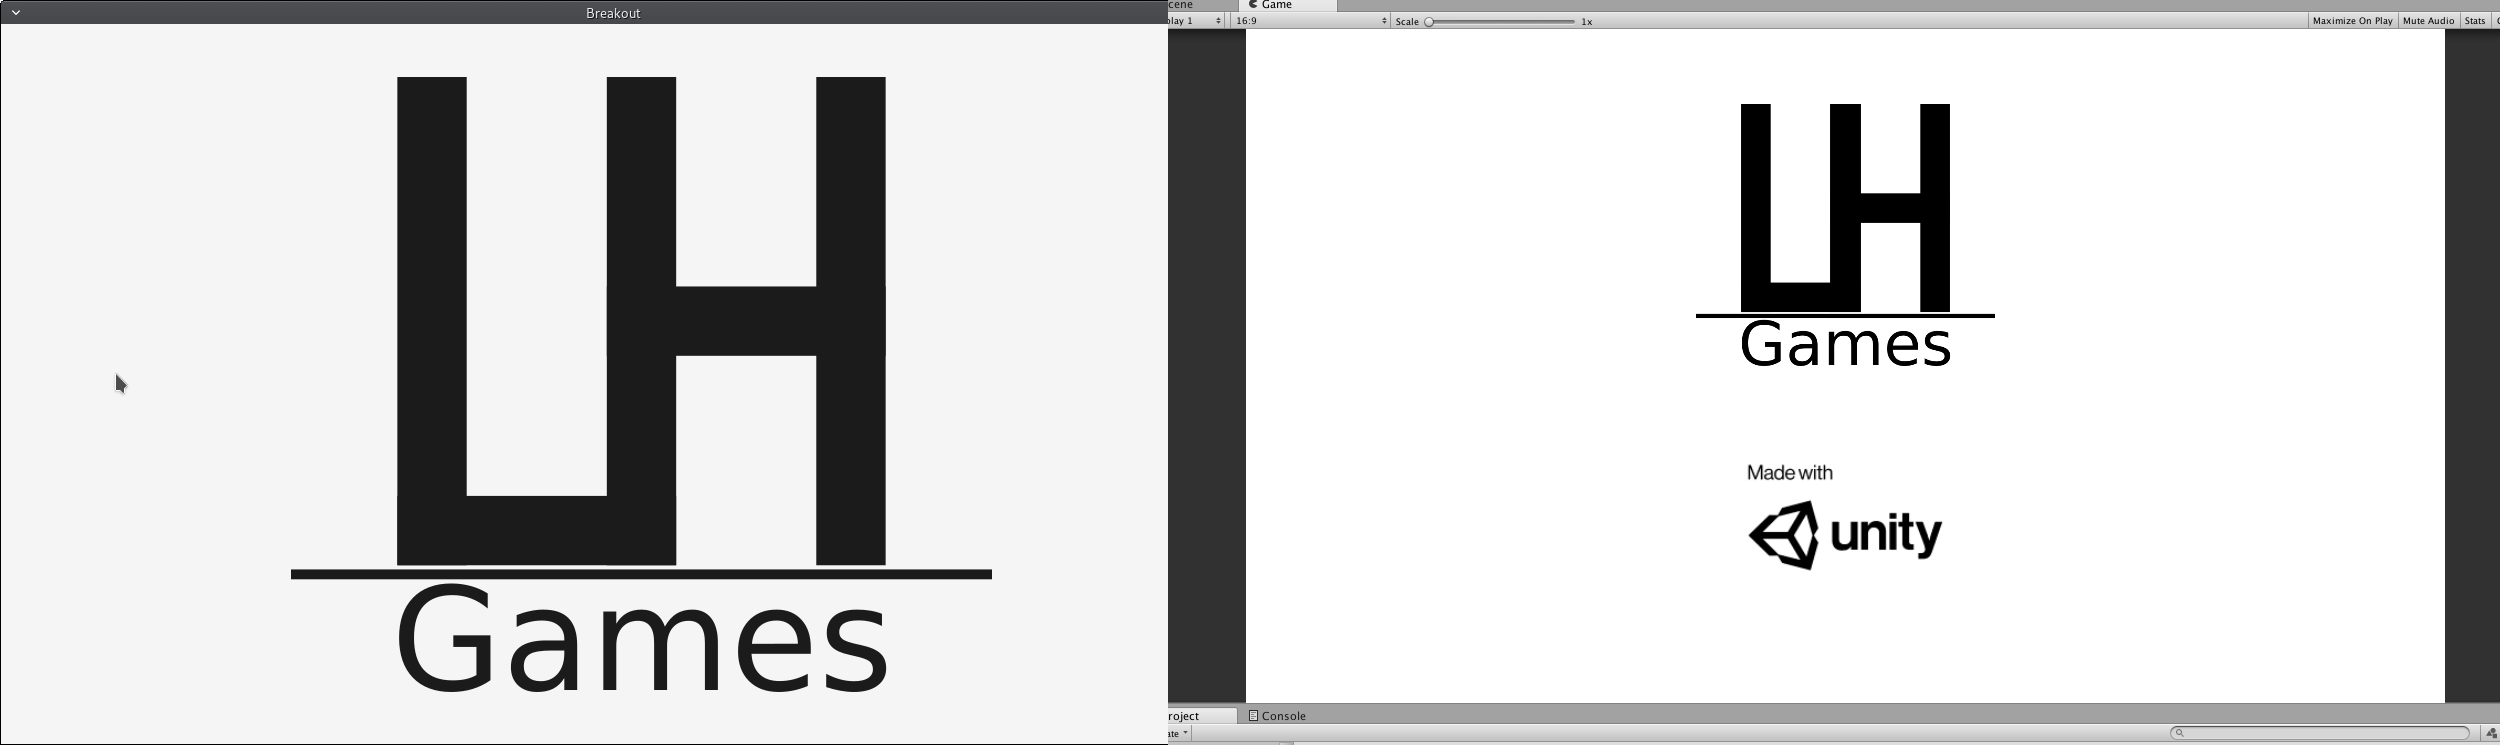
\includegraphics[width=14cm]{titleScreen}
	\caption{Naslovni zaslon. Levo v RayLib in LibGDX, desno v Unity.}
	\label{slika:naslovniZaslon}
\end{figure}
\item Glavni meni igre viden na sliki \ref{slika:mainMenu}. V glavnem meniju prikažemo naslov igre in nekaj dodatnih slik za popestritev scene. Uporabnik ima nato na voljo izbrati začetek igre ali zapustiti aplikacijo.
\begin{figure}[h]
	\centering
	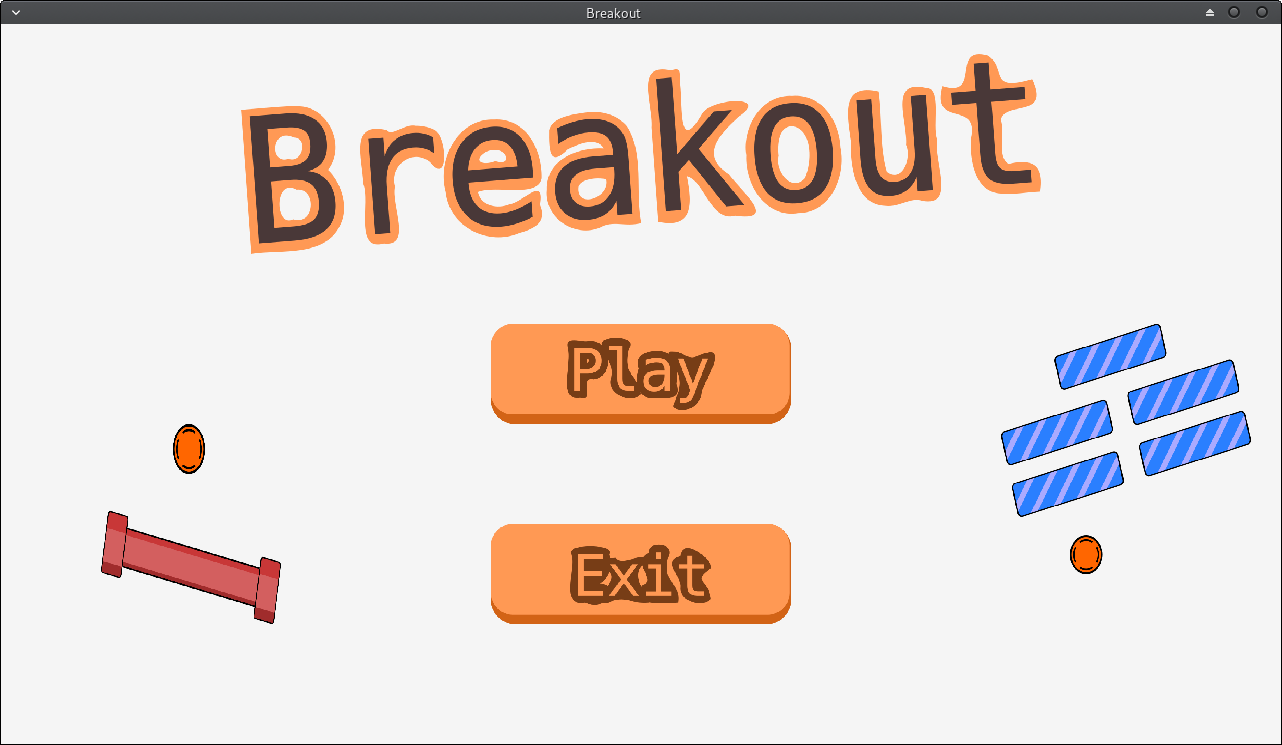
\includegraphics[width=14cm]{mainMenu}
	\caption{Glavni meni igre}
	\label{slika:mainMenu}
\end{figure}
\item Igralni del igre, ki je implementiran po zgornjem opisu. Z RayLib in LibGDX smo igro implementirali v 2D pogledu, kjer smo uporabili brezbarvne grafične gradnike, ki smo jih nato lahko individualno barvali med igranjem. V pogonu Unity  smo igro implementirali v 3D pogledu z modeli, ki smo jih izdelali sami. Oba pogleda lahko vidimo na slikah \ref{slika:2dGame} in \ref{slika:3dGame}.
\begin{figure}[h!]
	\centering
	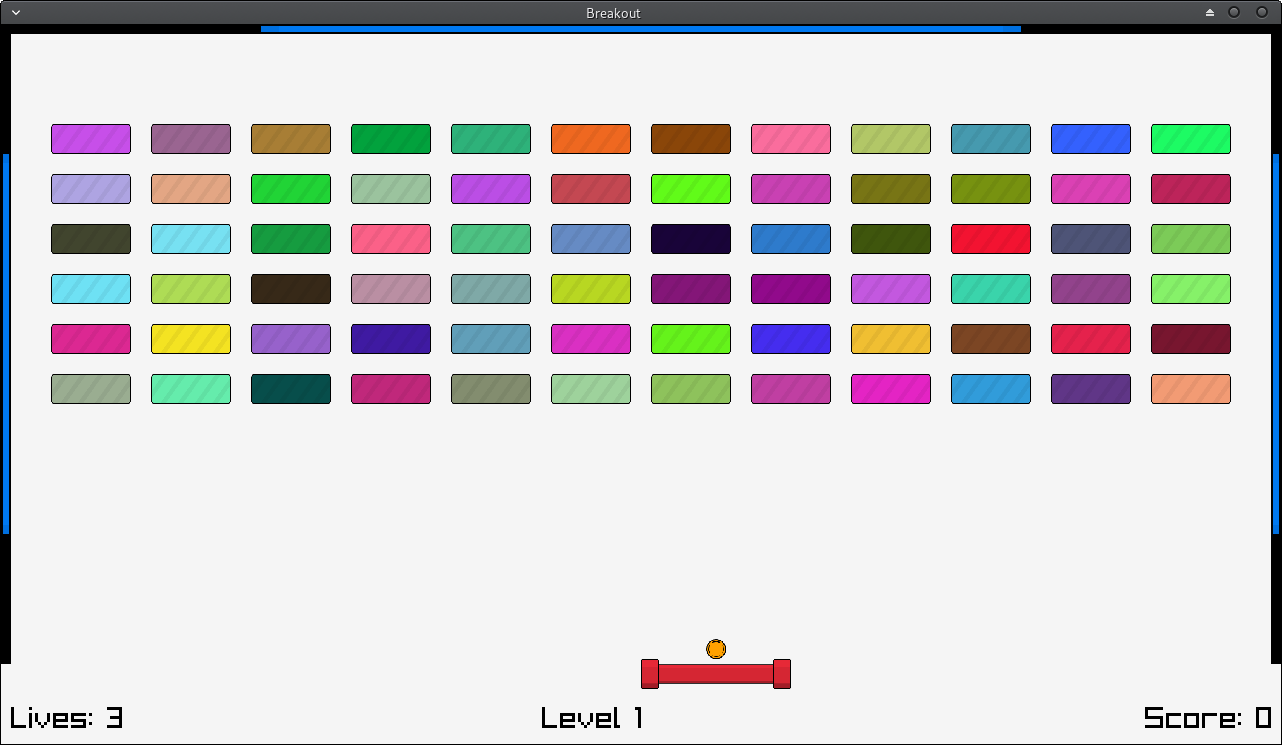
\includegraphics[width=14cm]{2dGame}
	\caption{2D variacija igre.}
	\label{slika:2dGame}
\end{figure}
\begin{figure}[h!]
	\centering
	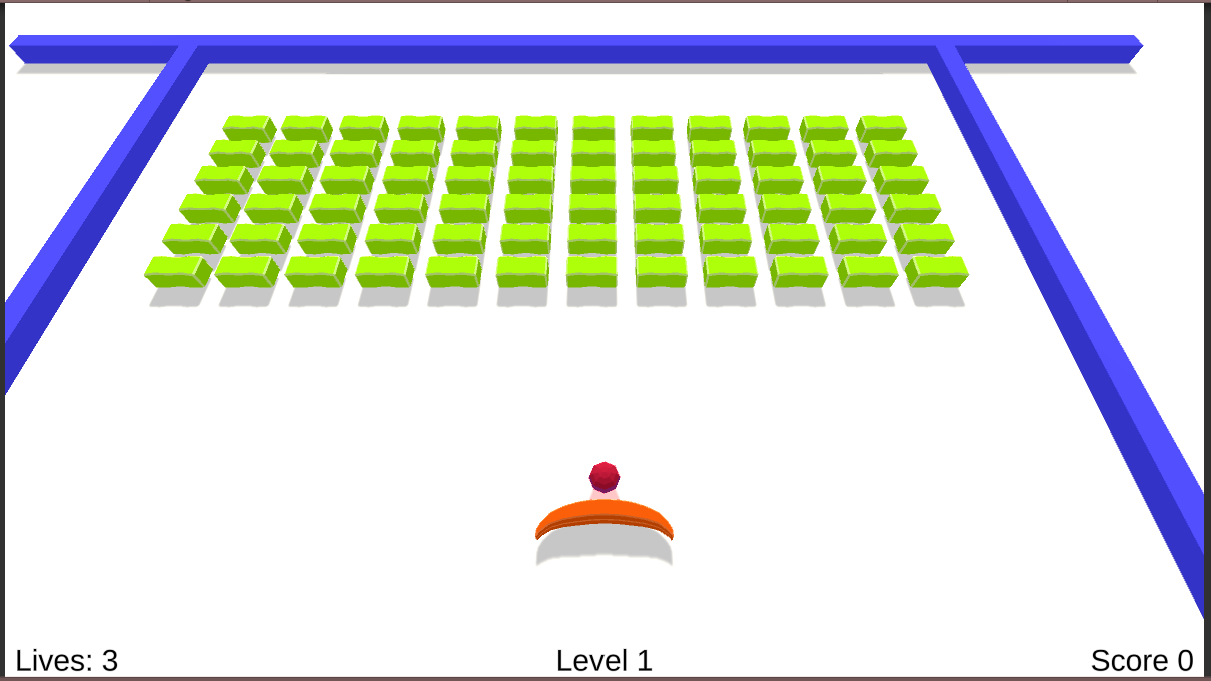
\includegraphics[width=14cm]{3dGame}
	\caption{3D variacija igre.}
	\label{slika:3dGame}
\end{figure}
\item Premikanje neodvisno od hitrosti izvajanja. Naše igre se obnašajo enako, neodvisno od zmogljivosti računalnika, na katerem se izvajajo.
\item Prehode med scenami z uporabo končnih avtomatov.
\item Upravljanje z grafičnimi in zvočnimi gradniki z direktorjem virov.
\item Prilagajanje izbrani ločljivosti. Neodvisno od uporabnikovega zaslona se naše igre prilagodijo brez rezanja prikazane vsebine.
\end{itemize}

Preostale funkcionalnosti, kot so na primer teksturni atlas, fizikalni pogoni ipd. smo implementirali samo v izbranih verzijah igre, saj niso tako korenito pomembne za razvoj. Vse uporabljene prakse in metode pa smo opisali v sledečih poglavjih magistrskega dela.

\section{Metode in prakse izdelave grafičnih gradnikov}
\subsection{Barvno neodvisni slikovni gradniki}
Izdelavo 2D gradnikov si lahko olajšamo z omejitvijo barv, tako da uporabljamo samo sivine. Take slike so potem neodvisne od barve in jim lahko programsko izberemo barvo med izvajanjem same igre. S tem si prihranimo čas, če se določeni objekti med sabo razlikujejo samo po barvah (npr. preprosti nasprotniki, ovire v igri ipd.). Spremembo barve v igri pa dosežemo z metodami za niansiranje.

V naši igri so vsi gradniki v 2D pogledu igre izdelani s to metodo. V sliki \ref{slika:grayscaleSprites} vidimo izdelane gradnike (od spodaj: lopar, ovira, žoga in desno zid) in v sliki \ref{slika:2dGame} vidimo končno uporabo v igri. Ovire v igri tvorijo lepo barvno paleto, v resnici pa je uporabljen samo en grafični gradnik. Sprememba barve loparju in žogi je tudi trivialna, saj gradnika ni potrebno znova barvati v izbranem orodju. 

\begin{figure}[h]
	\centering
	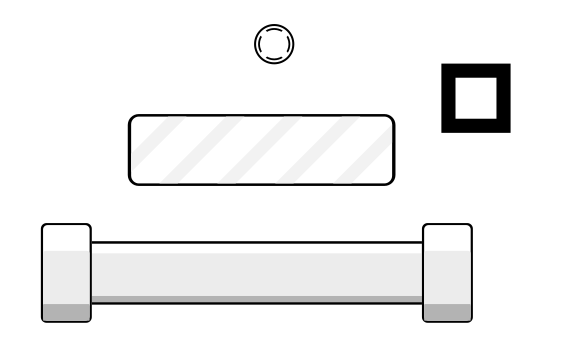
\includegraphics[width=8cm]{grayscaleSprites}
	\caption{2D sivinski gradniki}
	\label{slika:grayscaleSprites}
\end{figure}

Vsako orodje ponuja metode za niansiranje slik. Velikokrat izbrano barvo podamo kar v izrisovalno metodo. V RayLib nam metoda \textit{DrawTexturePro} ponudi šesti parameter, kamor vnesemo izbrano barvo. Primer lahko vidimo v izseku kode \ref{code:assetManager} v poglavju \ref{section:upravljanje}. Če bi uporabljali barvno sliko, potem podamo v metodo belo barvo in s tem ne vplivamo na barvno nianso našega gradnika. V LibGDX niansiranje kontroliramo izven izrisovanja individualne slike. Razred \textit{SpriteBatch}, ki ga uporabljamo za izrisovanje, ponuja metodo \textit{setColor(color)}, s katero izberemo nianso za vse nadaljnje izrise. Poskrbeti moramo le, da po uporabi nianso ponovno nastavimo na belo in s tem ne pokvarimo preostalega izrisovanja.

Unity nam ponuja dva načina za niansiranje barv izrisovanja. Neodvisno ali pa za izrisane 2D ali 3D gradnike potrebujemo material, ki določa lastnosti izrisovanja. Ena izmed lastnosti je niansa barve. Težava pri tej metodi je, da hočemo zaradi optimizacije uporabljati čim manj različnih materialov, ki pa so potrebni, da individualno nastavljamo nianse. Pri tem se moramo odločiti, ali je bolj pomembna hitrost izrisovanja ali niansiranje sivinskih gradnikov. Malo število nians oziroma materialov ne predstavlja velikega napora za Unity, vendar se moramo zavedati mogočih posledic pri množični uporabi. Drugi način niansiranja je možen samo za 2D gradnike in je neodvisen od materialov. \textit{Sprite Renderer} komponenta, ki se uporablja za izrisovanje 2D gradnikov, ponuja lastnost nianse slike, ki jo lahko uporabimo za naše namene. To lastnost lahko uporabljamo brez vpliva na zmogljivost, vendar smo omejeni samo na 2D slike.

\subsection{Teksturiranje modelov z barvnimi paletami}
Teksturiranje modelov je obsežen proces, ki zahteva več korakov. Najprej je potrebno površino modela UV mapirati (U in V sta osi na 2D teksturi, ki so jih uporabili, ker sta X in Y že uporabljena za definicijo lokacije modela v prostoru) na 2D sliko brez vidnih deformacij, nato pa na to sliko narisati želeno teksturo. Z mapiranjem prenesemo vsako ploskev modela na 2D površino. S tem postopkom dobimo za vsak model svojo teksturo, ki jo uporabimo pri izrisovanju. Pri kompleksnih modelih je tak postopek zaželen, ko pa izdelujemo preprostejše modele (angl. \textit{low poly}), želimo ploskve modela preprosto obarvati z izbrano barvo. Takrat je prej omenjen postopek zamuden in potraten, obenem pa zaradi individualnih tekstur za vsak model izgubimo na zmogljivosti izrisovanja. Zato lahko pri preprostih modelih uporabimo metodo teksturiranja z barvnimi paletami.

Metoda za teksturo uporablja barvno paleto z naborom barv za vse naše modele. Tako lahko uporabimo eno samo teksturo za vse naše modele. Mapiranje modelov pri tej metodi je zelo preprosto, saj moramo individualne poligone modela mapirati v območje izbrane barve v teksturi. Na sliki \ref{slika:texturePalette} vidimo, da poligona ni potrebno točno mapirati, saj nam večji del teksture predstavlja izbrano barvo. 

\begin{figure}[h]
	\centering
	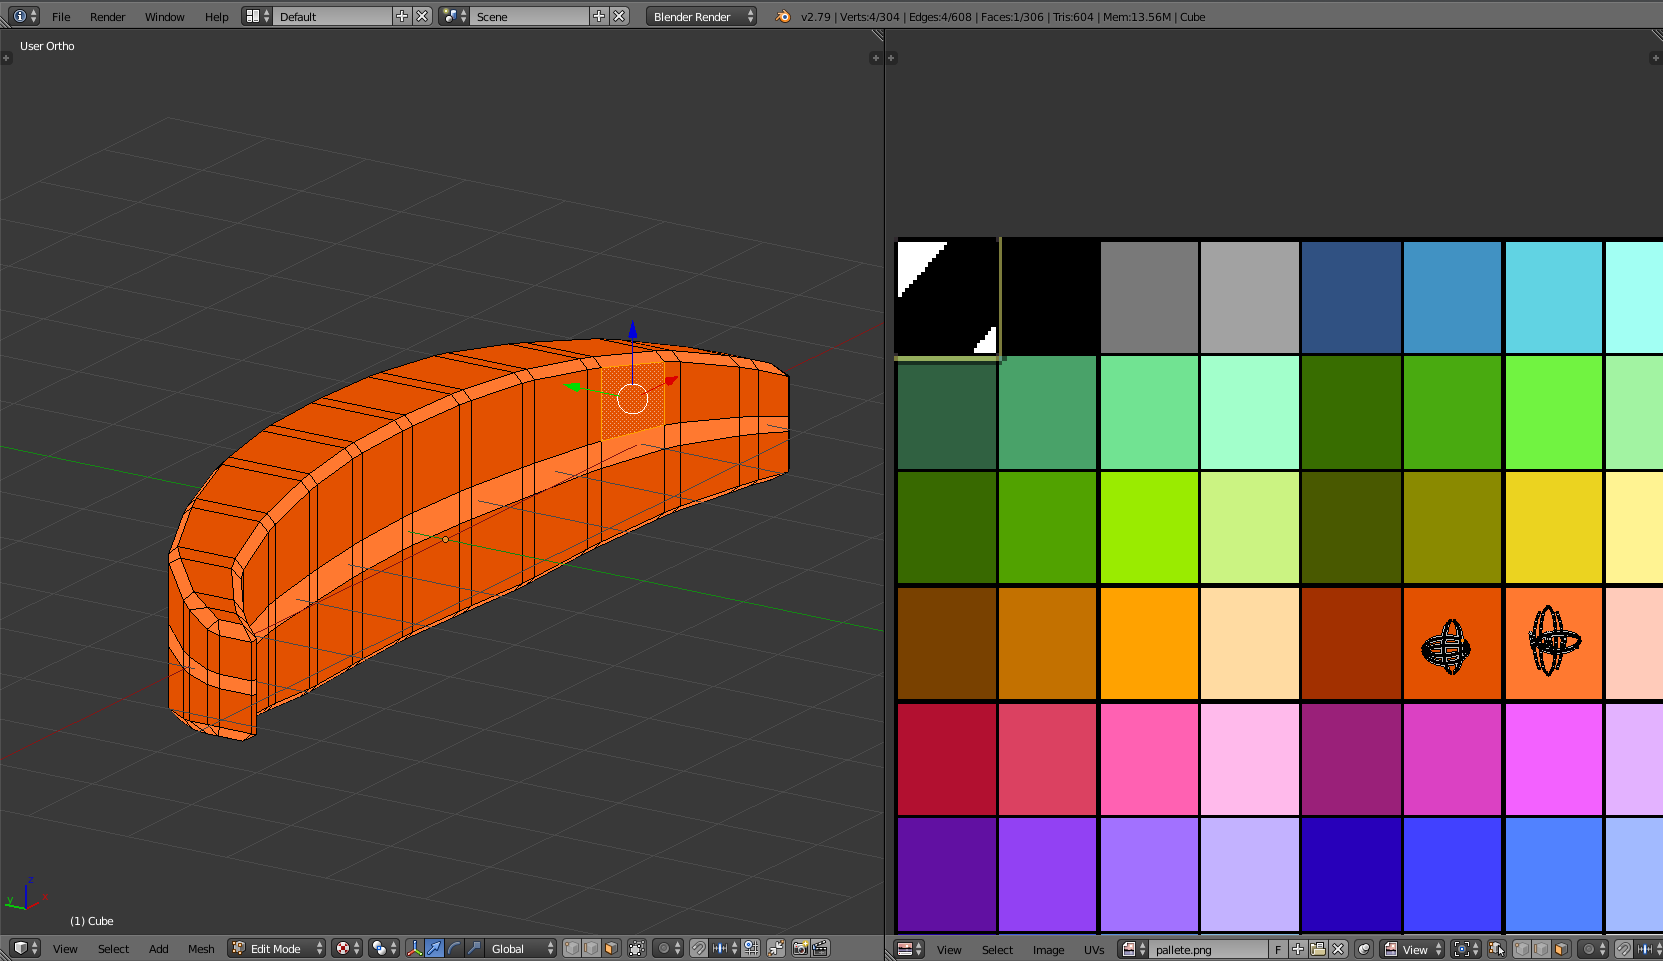
\includegraphics[width=14cm]{texturePalette}
	\caption{Mapiranje UV preprostih modelov}
	\label{slika:texturePalette}
\end{figure}

S to metodo smo izdelali vse modele za našo igro. V pogonu Unity smo potrebovali samo en material za izrisovanje vseh modelov, zato je ta metoda zelo učinkovita. Obenem metoda nudi dve veliki prednosti za spreminjanje barv med igro. Ker uporabljamo sliko barvne palete, lahko to enostavno zamenjamo z drugo in tako preprosto zamenjamo barve na modelu ali celo na celotni sceni, če vsi modeli uporabljajo isto paleto. Tako lahko z enostavno menjavo dodamo večjo raznolikost našim stopnjam. Druga prednost te metode pa je lažje individualno menjavanje barv na modelu. Pri standardnem mapiranju se skoraj nikoli programsko ne spreminjajo UV lokacije oglišč, saj je mapiranje specifično za ta model. S to metodo je mogoče zaznati oglišča, ki se nahajajo na izbrani barvi v teksturi in jih premestiti na drugo barvo. Tako lahko izbranemu objektu spremenimo izbrane barve. Je pa tako menjavanje omejeno na vse poligone enake barve v modelu, saj ni mogoče spremeniti barve samo enemu poligonu.

\section{Osnovne metode in prakse}
Ne glede na izbiro orodij za tehnično implementacijo računalniške igre, so določene metode in prakse skupne vsem. Tudi če orodje poskrbi za določene prakse, je dobro, da se jih zavedamo in tako bolje razumemo delovanje naših orodij in lahko bolj učinkovito implementiramo našo igro.

\subsection{Glavna zanka igre}
Glavna zanka igre skupaj z neodvisnim gibanjem od hitrosti izvajanja sta dva koncepta, ki sta specifična za igre ob izdelavi programske opreme. Nekatera programska oprema se izvede in nato prikaže svoje rezultate brez kakršnih koli vhodov, druga konstantno čaka na vhod ali dogodek od uporabnika, da proži akcije. Računalniške igre pa so konstantno v gibanju, tudi ko ne dobivajo vhoda od igralca. Če se igralec ustavi, se svet okoli njega v igri ne ustavi. Implementacija tega koncepta se imenuje glavna zanka igre. Psevdokodo preproste glavne zanke vidimo v izseku \ref{code:glavnaZanka}.

\begin{lstlisting}[label=code:glavnaZanka, language=C++, caption=Glavna zanka igre]
while(!shouldCloseGame)
{
	handleInput();
	update();
	render();
}
\end{lstlisting}

Kot vidimo, je glavna zanka sestavljena iz treh glavnih delov: pridobitev in procesiranje vhoda od igralca, simulacija sveta igre in izris stanja na zaslon. Zanka se izvaja, dokler se igralec ne odloči, da igro zapre. Zagotavlja, da konstantno preverjamo vhode od uporabnika, odzovemo svet igre glede na ta vhod in nato takoj damo povratne informacije igralcu preko izrisa na zaslon. Za merjenje hitrosti izvajanja glavne zanke večinoma uporabljamo mero sličic na sekundo (angl. \textit{frames per second}), ki nam pove, kolikokrat na sekundo se posodobijo informacije na zaslonu preko izrisa.

\subsection{Gibanje neodvisno od hitrosti izvajanja}
Hitrost izvajanja glavne zanke igre je zelo odvisna od specifikacij, ki jih premore strojna oprema, na kateri igro izvajamo. Obremenjenost opreme je tudi faktor, če poleg igre izvajamo še druge procese. Tehnologija osveževanja zaslonov lahko tudi umetno omejuje hitrost izrisovanja in posledično tudi hitrost izvajanja glavne zanke. Dandanes igre ciljajo dve hitrosti: to sta 30 ali 60 sličic na sekundo, odvisno od tehnične zahtevnosti igre in ciljne platforme, saj konzole niso tako zmogljive kot namenski igralski računalniki. Ciljno hitrost najlažje dosežemo z umetnim čakanjem za izrisom. 

Neodvisno od ciljne hitrosti pa v igri prihaja do nihanj. Določene scene zahtevajo več računalniških virov in tako povečajo potrebno procesorsko moč. Takrat se hitrost izvajanja zanke upočasni. Pri osnovnem modelu glavne zanke oziroma pri modelu z umetnim čakanjem bi to pomenilo upočasnitev same igre. Svet bi se simuliral počasneje in igralcu bi se zazdelo, kot da vse poteka v počasnem posnetku. Da se temu izognemo, uporabljamo metode, ki simulirajo igro z enako hitrostjo, neodvisno od hitrosti izvajanja glavne zanke. Najbolj priljubljena metoda uporablja merjenje časa, ki je pretekel od prejšnje izvedbe glavne zanke. Primer psevdokode vidimo v izseku \ref{code:deltaTime}.

\begin{lstlisting}[label=code:deltaTime, language=C++, caption=Neodvisno gibanje]
float previousTime = getCurrentTimeInMs();
while(!shouldCloseGame)
{
	float currentTime = getCurrentTimeInMs();
	float deltaTime = (currentTime - previousTime) / 1000.0f;
	handleInput();
	update(deltaTime);
	render();
	previousTime = currentTime;
}

void update(float deltaTime)
{
	position.x += 200 * deltaTime; //Hitrost premikanja je 200 enot na sekundo
}
\end{lstlisting}
Kot vidimo, si izračunamo delta čas med ponovitvami zanke. Dobra praksa je delto pretvoriti v sekunde, saj jo potem lažje uporabljamo v računske namene. Delta čas podamo v metodo, kjer se izvaja simulacija, in ga uporabimo pri operacijah, ki so odvisne od hitrosti izvajanja. Tako lahko dosežemo, da se premikamo s konstantno hitrostjo na sekundo, ne glede na hitrost izvajanja glavne zanke.

Razvojna orodja nam ponujajo različne načine upravljanja z glavno zanko in delta časom. Pri nizkonivojskem programiranju si moramo sami ustvariti glavno zanko in se odločiti, kako se bo prožilo zaporedje dogodkov. Knjižnica Raylib nam ponuja metodo \textit{GetFrameTime()}, ki nam vrne delta čas v sekundah. Pri tako dostopni metodi moramo paziti, da delta čas pridobimo samo enkrat v eni ponovitvi zanke. Če bi čas pridobili na več mestih, bi bil ta lahko različen in bi se objekti v naši igri simulirali z različnimi hitrostmi. Zato je ustaljena praksa, da čas pridobimo enkrat in ga nato predamo v nadaljnje metode.

Ogrodje LibGDX ima točno definirano glavno zanko, na katero ne moremo vplivati. Implementirati moramo vmesnik \textit{ApplicationListener}, ki nam ponuja samo eno vstopno točko v zanko, metodo \textit{render()}. Ime metode je zavajajoče, saj ni namenjena samo za izrisovanje. Uporabiti jo moramo kot telo glavne zanke in v njej implementirati simulacijo igre in izrisovanje. Procesiranje vhodov se v LibGDX izvaja s proženjem dogodkov, ki potekajo neodvisno od metode \textit{render()}. Za pridobitev delta časa nam je podobno kot pri Raylib na voljo metoda \textit{Gdx.graphics.getDeltaTime()}.

Pogon Unity ima zelo kompleksno glavno zanko razdeljeno na več delov (simulacija fizikalnega pogona, proženje dogodkov, simulacija igre, izrisovanje scene, izrisovanje uporabniškega vmesnika ipd.). Z našimi objekti se lahko vključimo v vsak posamezen korak glavne zanke. Unity poleg simulacije igre izvaja še simulacijo fizikalnega pogona, ki se lahko izvede večkrat v eni iteraciji glavne zanke. Metodi za delo s simulacijama sta \textit{FixedUpdate()} (simulacija fizikalnega pogona) in \textit{Update()} (preostala simulacija). Za pridobitev delta časa nam je na voljo metoda \textit{Time.deltaTime()}.

\subsection{Upravljanje stanj v igri}
Upravljanje stanj je mišljeno kot organizacija in prehajanje med stanji, kot so začetni logotip, različni meniji igre (glavni meni, meni za izbiro stopenj ipd.) in različnimi nivoji igre. Stanja so uporabna, saj lahko ločimo našo igro na individualne dele, ki se izvajajo neodvisno na druga stanja. Za stanja se uporablja tudi sinonim scena. Vsako ogrodje in namenski pogon ima svoj način dela s stanji, vendar so večinoma to preprosti končni avtomati, ki imajo definirane prehode med scenami in hranijo vsak svoje interne objekte. Ti interni objekti so potem gradniki, uporabljeni v sceni igre. Med samo igro je to igralec in objekti v svetu, v meniju so gradniki grafičnega vmesnika, ki se odzivajo na dogodke ipd.

Pri nizkonivojskih knjižnicah smo sami implementirali prehode med scenami. Za osnovo potrebujemo abstraktni razred, ki bo ogrodje za glavne metode scene (deli glavne zanke igre). Primer vidimo v izseku \ref{code:stanjeIgre}.

\begin{lstlisting}[label=code:stanjeIgre, language=C++, caption=Stanje igre]
enum GameStates {STATE_NULL, STATE_TITLE, STATE_LEVEL, STATE_EXIT};

class GameState {
	protected:
		GameStates currentGameState = GameStates::STATE_NULL;
		GameStates nextGameState = GameStates::STATE_NULL;
	public:
		virtual ~GameState();
		virtual void handleEvents() = 0;
		virtual void handleLogic(const float deltaTime) = 0;
		virtual void handleRendering() = 0;
		GameStates getNextState() const;
		void changeGameState(const GameStates state);
};
\end{lstlisting}

Pri taki zasnovi smo nato preprosto dedovali od razreda \textit{GameState} in implementirali individualna obnašanja scen. Vsaka scena poskrbi za konstrukcijo in destrukcijo svojih objektov, med sabo pa si delijo skupne vire (kot recimo grafični in glasbeni gradniki). V glavni metodi naše aplikacije smo z uporabo polimorfizma ustvarili instanco enega stanja igre ter preprosto klicali namenske metode glavne zanke (izsek \ref{code:uporabaStanja}). V metodo za simulacijo igre smo podali delta čas, ki smo ga omenili v prejšnjem poglavju. Tako smo poskrbeli, da je delta čas enak skozi celotno simulacijo v enem koraku.

\begin{lstlisting}[label=code:uporabaStanja, language=C++, caption=Uporaba stanja igre]
std::unique_ptr<GameState> currentState = std::make_unique<LevelState>();

while (currentState->getNextState() != STATE_EXIT) {
	currentState->handleEvents();
	currentState->handleLogic(GetFrameTime());
	currentState->handleRendering();
	if (currentState->getNextState() != STATE_NULL) switchGameState(currentState);
} //...
\end{lstlisting}

Ogrodje LibGDX nam ponuja vmesnik \textit{Screen}, ki deluje podobno kot naš implementiran \textit{GameState} razred. Upravljanje s scenami smo morali implementirati sami, saj ogrodje nima implementiranega svojega načina. Pri tem smo upoštevali enake principe kot pri nizkonivojski knjižnici. LibGDX nam olajša prehode med scenami, saj razred \textit{Game} ponuja metodo \textit{setScreen}, ki enostavno uniči trenutno sceno in naloži novo. Mi smo samo implementirali transformacije, kdaj se katera scena spremeni v drugo.

Unity ima svoj sistem upravljanja s scenami, vendar je v ozadju zelo podoben temu v LibGDX. V grafičnem urejevalniku smo ustvarili posamezne scene in jih shranili s končnico \textit{.unity}. Vse možne scene nato naštejemo v nastavitvah naše aplikacije, nakar nam Unity ponudi singleton \textit{SceneManager} za upravljanje prehodov. Dve glavni metodi za prehode med scenami sta \textit{LoadScene} in \textit{LoadSceneAsync}. Znotraj podamo ime scene, pogon jo naloži in nato zamenja obstoječo sceno. Razlika med metodama je v tem, da prva blokira izvajanje med nalaganjem, druga pa naloži sceno v ozadju. Privzeto se celotna obstoječa scena zamenja z novo, ponuja pa Unity nalaganje scen ene v drugi. Tako lahko naložimo več različnih scen in jih združimo v želeno celoto. Ta princip je uporaben, če imamo del scene vedno enak (statičen, recimo igralčev lik), pri preostanku scene pa so možne različne variacije.

\subsection{Ločljivost igre}
Zasloni, na katerih se bo naša igra prikazovala, imajo različne ločljivosti in razmerja med horizontalno ter vertikalno dolžino. Te razlike lahko privedejo do nepričakovanih sprememb pri izrisovanju, če razlik nismo predvideli. Najhuje je, ko se del scene ne izriše, ker je ločljivost igre ožja od pričakovane. Primer lahko vidimo na sliki \ref{slika:rezanje}. S črno obrobo je prikazana ločljivost zaslona oziroma okna igre, s temno rdečo pa scena. Prvi primer prikazuje optimalno izrisovanje, primera 2 in 3 pa težave, ki nastanejo, če ne poskrbimo za različne ločljivosti. Kot vidimo iz slike, določeni deli scene niso več videni na zaslonu.

\begin{figure}[h]
	\centering
	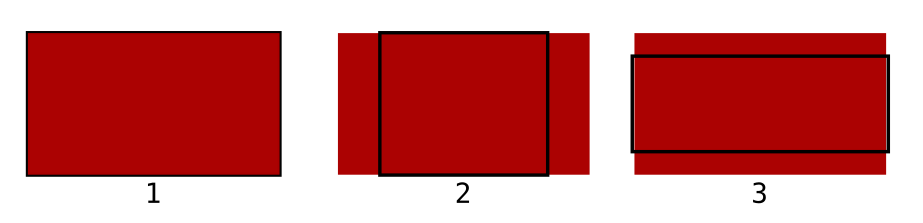
\includegraphics[width=12cm]{rezanjeResolucije}
	\caption{Primeri izgubljenega dela scene.}
	\label{slika:rezanje}
\end{figure}

Za reševanje teh težav nam orodja večinoma ponujajo delo s kamerami ali pogledi na sceno. Z njimi lahko krmilimo, kako se bo izrisovanje odzivalo na različne ločljivosti. Ko igro razvijamo, jo večinoma zasnujemo z določeno ločljivostjo in razmerjem v mislih, nato pa poskrbimo za potrebna prilagajanja. Na voljo imamo več načinov: moramo se odločiti, ali bomo ohranjali razmerje ali ne. Če originalnega razmerja ni potrebno ohranjati, potem lahko izrisovanje prilagodimo novi ločljivosti in izris preprosto raztegnemo na uporabnikovem zaslonu. Pri tem lahko pride do popačenj, vendar vedno zapolnimo razpoložljivo ločljivost. Če hočemo ohranjati originalno razmerje, pa moramo skleniti določene kompromise. Ti kompromisi so črni oziroma prazni deli zaslona, saj če se uporabnikovo razmerje dimenzij ne sklada z zasnovano, potem ni mogoče popolnoma prilagoditi izrisovanja. Primera prilagajanja vidimo na sliki \ref{slika:prilagajanje}. V primeru 1 je uporabnikova ločljivost ožja od zasnovane, zato smo izris prilagodili. Zaradi ohranjanja originalnega razmerja imamo na vrhu in dnu zaslona prazne dele. Primer 2 prikazuje ravno nasproten scenarij.

\begin{figure}[h]
	\centering
	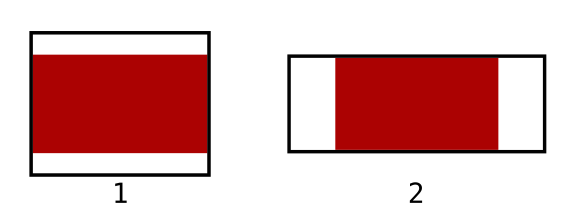
\includegraphics[width=10cm]{prilagajanje}
	\caption{Primeri prilagajanja izrisovanja.}
	\label{slika:prilagajanje}
\end{figure}

Knjižnica RayLib ponuja razred \textit{Camera2D} za upravljanje z ločljivostjo. Podpira samo prilagajanje z ohranjanjem razmerja, saj ni mogoče neodvisno spreminjati horizontalne in vertikalne povečave, ampak le s skupnim faktorjem preko \textit{zoom} spremenljivke. Kameri nato postavimo še izvirno velikost in položaj ter jo uporabimo pred začetkom izrisovanja z metodo \textit{Begin2dMode()}. Ko zaključimo izrisovanje, uporabimo metodo \textit{End2dMode()}. Ti metodi poskrbita, da se vso izrisovanje prilagodi parametrom kamere.

LibGDX ogrodje ponuja veliko bolj dovršen način upravljanja z ločljivostjo z uporabo razredov \textit{Camera} in \textit{Viewport}. Na voljo nam je več specializacij razreda \textit{Viewport}. \textit{StretchViewport} prilagaja ločljivost brez ohranjanja originalnega razmerja, \textit{FitViewport} pa ohranja razmerja, vendar pušča prazne predele. Obstaja še \textit{FillViewport}, ki podobno kot \textit{FitViewport} ohranja razmerje, vendar ne pušča praznih predelov, temveč poveča izris izven zaslona, tako da določeni deli scene niso vidni. Uporaba razredov je preprosta, saj jih le ustvarimo z želeno originalno ločljivostjo, nato pa podobno kot pri RayLib uporabimo metodo \textit{setProjectionMatrix} pred izrisovanjem.

Unity ponuja kamera objekte za prilagajanje ločljivosti. Igre v Unity so vedno 3D, tudi kadar uporabljamo 2D komponente, zato kamere delujejo za 3D svet. To pomeni, da ni mogoče na enostavni način prilagajati izrisovanja z ohranjanjem originalnega razmerja. Če hočemo ohranjati razmerje, je potrebno v izrisovanje vključiti vmesni korak: to je izrisovanje na teksturo, katero nato prilagodimo in jo prikažemo na zaslonu. Če pa nočemo ohranjati razmerja in prilagoditi originalni izris kakršni koli ločljivosti, pa enostavno nastavimo \textit{aspekt} komponento kameri na želeno originalno vrednost in Unity bo avtomatsko prilagodil izris.

\subsection{Upravljanje z grafičnimi in glasbenimi gradniki}
\label{section:upravljanje}
Upravljanje z grafičnimi in glasbenimi gradniki je pomemben del razvoja igra. Ti gradniki predstavljajo po velikosti največji del naše igre, zato se moramo odločiti, kako jih bomo uporabljali. Ker so ti gradniki veliki, jih nočemo nalagati med samim igranjem, saj lahko potem pride do nepotrebnih zastojev med igranjem. Nalaganje se večinoma dogaja na samem začetku pogona igre ali v vmesnih scenah, kjer so namenjeni specifično za to. Nalaganja med igranjem se poslužujemo samo v primeru, da so naši gradniki preveliki (ko velikosti začnejo dosegati gigabajte) -- takrat obstajajo tehnike za sprotno nalaganje.

V naših igrah gradniki niso bili preveliki, zato smo se odločili, da jih vse naložimo ob zagonu igre. Pogon Unity dela z gradniki drugače in jih naloži takrat, ko nalagamo sceno, v kateri je gradnik uporabljen. Neodvisno od uporabljene strategije pa je pomembno, da gradnike ločimo od drugih komponent v naši igri in jih naložimo samo enkrat. Če bi gradnik vezali na objekt v igri, kot na primer strelivo, bi konstantno prihajalo do nalaganja in odlaganja grafičnega gradnika, ko bi igralec streljal, čez čas pa bi strelivo izginilo zaradi optimizacije. Takega delovanja si ne želimo, saj hočemo, da je isti grafični gradnik uporabljen za vso strelivo. Za takšno upravljanje uporabljamo princip direktorja virov, ki hrani vse potrebne gradnike in jih daje na voljo drugim objektom. Velikokrat se ti direktorji poslužujejo singleton principa, saj nočemo več instanc direktorja virov.

V C++ smo si sami ustvarili direktorja, saj knjižnica Raylib ne ponuja take funkcionalnosti. Naš direktor je hranil mapo tekstur in zvokov, do katerih smo dostopali preko imen, ki smo jih priredili gradnikom. Direktor je bil singleton, ki je bil na voljo vsem objektom v igri. Nalaganje gradnikov smo izvršili pred začetkom glavne zanke igre. V izseku \ref{code:assetManager} vidimo primer uporabe. Prvi dve vrstici prikazujeta nalaganje gradnikov pod izbranim imenom, tretja vrstica pa prikazuje kasnejšo uporabo pri izrisovanju. 

\begin{lstlisting}[label=code:assetManager, language=C++, caption=Uporaba direktorja virov]
AssetManager::getInstance().loadTexture("pad", "../assets/pad.png");
AssetManager::getInstance().loadSound("blip", "../assets/blip.wav");
DrawTexturePro(AssetManager::getInstance().getTexture("wall"), AssetManager::getInstance().getRectangle("wall"), renderRectangle, Vector2{0, 0}, 0, BLUE);
\end{lstlisting}

Ogrodje LibGDX ponuja direktorja že v svoji funkcionalnosti pod imenom \textit{AssetManager}. Ponuja metodi \textit{load(path, type)} in \textit{get(path, type)}, ki upravljata z gradniki. V LibGDX direktor privzeto ni singleton, zato ga nismo spreminjali. Prvotno smo ga ustvarili v vhodni metodi v igro in si instanco predajali med scenami ter na koncu tudi v metode samih objektov, ki so potrebovali gradnike (npr. za izrisovanje). Druga pomembna razlika direktorja v LibGDX je, da gradnike nalaga asinhrono, pri čemer Raylib nalaga sinhrono. V LibGDX lahko z metodo \textit{finishLoading()} direktorja prisilimo, da dokonča nalaganje, preden nadaljujemo z izvajanjem, in se tako izognemo napakam zaradi nepopolnega nalaganja.

Pogon Unity, kot že omenjeno, dela drugače z gradniki. V ozadju naloži gradnike, ko pride do nalaganja same scene. Gradniki so v urejevalniku direktno povezani z objekti v igri, vendar v ozadju Unity poskrbi, da so to dejansko isti gradniki in da ne pride do nepotrebnega nalaganja in odlaganja. Za naknadno nalaganje Unity ponuja dva mehanizma. Prvi je posebno imenovana mapa \textit{Resources}, kjer shranimo gradnike, ki jih bomo uporabljali za ta namen. Nato lahko med izvajanjem uporabljamo sinhrono metodo \textit{Resources.Load(name, type)} ali asinhrono metodo \textit{Resources.LoadAsync(...)}. Ko gradnikov več ne potrebujemo, jih lahko odložimo z metodo \textit{Destroy()} in \textit{Resources.UnloadUnusedAssets()}. Drugi način nalaganja gradnikov med izvajanjem so tako imenovani paketi sredstev (angl. \textit{asset bundle}). To so skupki večjega števila gradnikov, ki jih lahko ustvarimo v urejevalniku in uporabniku dostavimo neodvisno od igre. Tako lahko izdelamo dodatke ali popravke za našo igro, brez da bi bilo potrebno ponovno prevesti našo igro. Te pakete nato med izvajanjem igre naložimo z metodama \textit{AssetBundle.LoadAsset(name)} in \textit{AssetBundle.Unload()}. 

\subsection{Teksturni atlasi}
Teksturni atlasi so najbolj pogosta optimizacija slikovnih grafičnih gradnikov. Ti gradniki se uporabljajo pri 2D igrah kot grafični liki, pri 3D igrah pa kot teksture na modelih. Večje število gradnikov nam zaseda omejen pomnilnik na grafični kartici, obenem pa je za izrisovanje na zaslon najbolj optimalno, če čim več izrisov združimo skupaj v enega. Združevanje pa ni možno, če izrisi potrebujejo različne slikovne grafične gradnike. Zato je primerno, da te gradnike združimo v en večji grafični gradnik, iz katerega potem preberemo le tisti del, ki ga potrebujemo. Ker pa ni potrebno menjati gradnika v ozadju, lahko take izrise združimo v enega. Temu principu rečemo teksturni ali slikovni atlas.

Prvi korak za uporabo teksturnih atlasov je sama njihova izdelava. Lahko se odločimo, da ročno iz več manjših slik ustvarimo eno večjo, vendar je to potratno, saj za ta namen obstaja veliko različnih orodij. Orodja slike združijo na najbolj optimalen način, tako da na teksturnem atlasu ostane čim manj neizkoriščenega prostora. Prazen prostor po nepotrebnem troši spomin grafične kartice, zato ga želimo minimizirati. Ogrodje LibGDX ponuja svoje orodje za izdelavo atlasov pod imenom GDX Texture Packer GUI\footnote{https://github.com/crashinvaders/gdx-texture-packer-gui}. S tem preprostim grafičnim vmesnikom izberemo slike, ki jih želimo zapakirati, nastavimo parametre obdelave in poženemo obdelavo. Z orodjem je obenem možno kontrolirati kakovost končne slike, algoritem pakiranja ipd. Orodje lahko vidimo levo na sliki \ref{slika:texturePacker}. Obenem nam poleg končne slike izdela še datoteko, ki hrani vse potrebne podatke za uporabo teksturnega atlasa.

Unity urejevalnik omogoča še enostavnejšo podporo teksturnim atlasom. Potrebno nam je samo omogočiti uporabo atlasov in nato specificirati, katere slike bodo uporabljene v atlasu. Unity potem avtomatsko poskrbi, da so izbrane slike uporabljene iz atlasov in tako uporabniku ni potrebno skrbeti za implementacijo. Kot vidno iz desnega dela slike \ref{slika:texturePacker} nam Unity prikaže, kakšen bo končni teksturni atlas.

\begin{figure}[h]
	\centering
	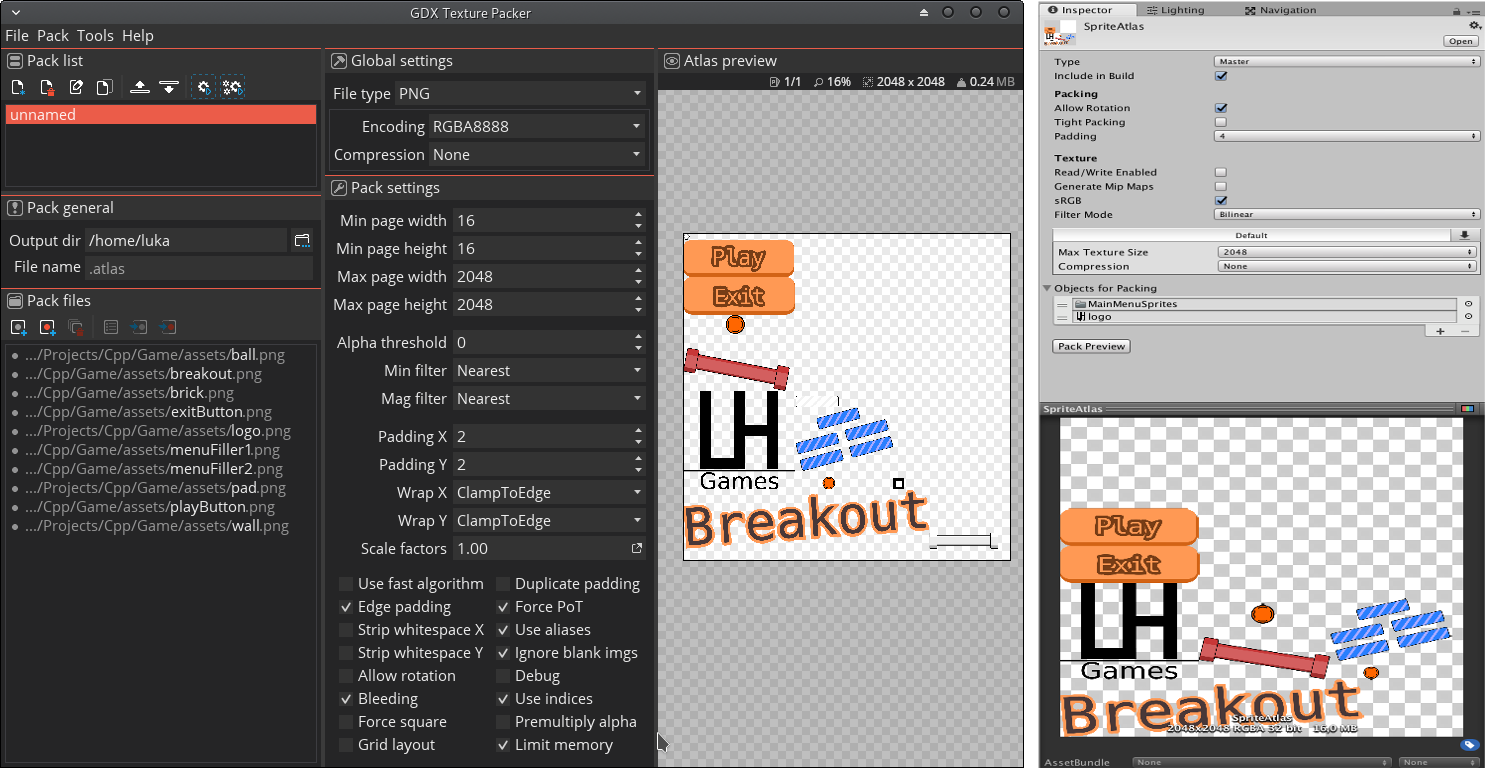
\includegraphics[width=15cm]{texturePacker}
	\caption{GDX Texture Packer GUI in Unity Sprite Packer}
	\label{slika:texturePacker}
\end{figure}
Uporaba teksturnih atlasov v Raylib in LibGDX zahteva dodatno delo za razliko od pogona Unity . Raylib nam ne ponuja nobene funkcionalnosti za podporo atlasov, tako da je potrebno implementirati uvoz ustvarjene datoteke z informacijami o atlasu. LibGDX pa ponuja potrebno funkcionalnost za delo z atlasi, ki so ustvarjeni z njihovim orodjem. Razred \textit{TextureAltas} nam omogoča branje ustvarjenih .atlas datotek, nakar nam ponuja metode, kot so \textit{findRegion(name)} in \textit{createSprite(name)}, da pridobimo ustrezne podatke za želeno izvorno sliko. Te informacije nato uporabimo pri izrisovanju podobno, kot da bi izrisovali posamezne slike. 

\section{Specifične metode in prakse}
Določene metode niso vsesplošno uporabljene v vseh orodjih za razvoj računalniških iger. Druge so na voljo samo v specifičnih orodjih kot je Unity. Kljub temu so zelo uporabne pri razvoju, zato smo jih opisali v tem poglavju.

\subsection{Fizikalni pogoni}
Za realistično simulacijo fizikalnih objektov potrebujemo fizikalni pogon. Kot že omenjeno, sta najbolj priljubljena pogona za 2D simulacijo Box2D in Chimpmunk. Za 3D simulacijo pa so med bolj znanimi Bullet, Physix in Havoc. Neodvisno od pogona pa pri vseh srečamo iste koncepte, prakse in gradnike, ki jih je potrebno razumeti za njegovo uporabo. Zato smo v našem delu opisali najbolj pomembne sklope pogonov:
\begin{itemize}
	\item \textbf{Simulacijski svet}.  Vsa simulacija se dogaja v tako imenovanem simulacijskem svetu. Ta je odgovoren za vsa telesa v simulaciji in nadzira dogajanje simulacije. Večinoma uporabljamo samo en simulacijski svet, saj interakcije med svetovi niso podprte. Svet se ne simulira samostojno in brez naše interakcije obstoji na miru, zato obstajajo specifične metode, s katerimi simulacijo poženemo naprej za določen čas. Klicanje teh metod vežemo na glavno zanko igre v simulacijskemu delu zanke. S svetovi tudi krmilimo glavne parametre fizikalne simulacije, kot so smer in moč gravitacije ter število iteracij pri reševanju trkov. Večje kot je število iteracij, bolj natančni in resnični so odzivi na trke.
	\item \textbf{Toga telesa (angl. \textit{rigid body})}. Toga telesa so osnova za vse objekte v fizikalnem svetu. Telesa ne predstavljajo oblike in velikosti objektov (to vlogo imajo konstrukcije), temveč lastnosti, kot so masa, hitrost  in smer gibanja, rotacijska inercija, rotacijska hitrost, lokacija in nagib. S pomočjo teh lastnosti in konstrukcije lahko nato razrešujemo trke med objekti.
	
	Vsi pogoni poznajo tri tipe togih teles: dinamične, statične in kinematične. Dinamična telesa predstavljajo vse objekte, kot jih poznamo v realnem svetu. Ti objekti se odzivajo na vse zunanje in notranje sile in se pri trkih realistično odzovejo. Dinamična telesa uporabljamo, ko hočemo simulirati realistično dogajanje v naši igri. Statična telesa ne obstajajo v realnem svetu, saj so to telesa, ki se na sile in trke ne odzivajo. Neodvisno od moči trka se ta telesa ne bodo premaknila (druga telesa se vedno odbijejo od njih), obenem jih ni možno premakniti v kodi. Statična telesa uporabljamo za statične dele nivojev v igri (tla, zid ipd.), za katere nočemo, da se premikajo, vendar morajo vseeno obstajati kot ovira za dinamična telesa. Kinematična telesa so zelo podobna kot statična telesa, le da jih je možno v kodi premikati po svetu. Ta telesa uporabljamo za neodzivne dele nivojev, ki pa se morajo premikati po določenih smernicah (npr. premikajoča tla).
	\item \textbf{Konstrukcija (angl. \textit{fixture}).} Konstrukcije so druga osnovna komponenta za fizikalno simulacijo. Predstavljajo obliko, velikost in materialne lastnosti objekta, priredimo pa jih na toga telesa. Odvisno od konstrukcije se telesu nato preračuna masa. Skupaj tvorijo predstavitev naših objektov v fizikalnem svetu. Lastnosti konstrukcije so gostota, trenje in moč odboja. Oblika konstrukcij je v veliko pogonih omejena na konveksna telesa. Ko hočemo simulirati konkavna telesa, uporabimo dve ali več konveksnih konstrukcij, ki jih priredimo enemu togemu telesu.
	\item \textbf{Sile in impulzi (angl. \textit{forces and impulses})}. Za realistično premikanje dinamičnih teles uporabljamo sile in impulze. Sile delujejo na telesa skozi čas, impulzi pa v trenutku prenesejo moč na telo. Oboje lahko uporabimo za premikanje po prostoru ter za rotacijo teles. Pri uporabi sil in impulzov vedno določimo moč in lokacijo, saj nočemo vedno uporabiti sile v centru mase objekta.
	
	Telesa lahko premikamo po svetu tudi z direktnim nastavljanjem lokacije. To ni realistično premikanje s pomočjo sil, zato lahko pride do nerealističnih odzivov drugih teles, kadar pride do trkov. Direktnemu premikanju se je zato najboljše izogniti in uporabljati sile in impulze. V realnem svetu se vse premika z njihovo pomočjo, zato si lahko prihranimo neznane težave pri simulaciji z izogibanjem direktnemu premikanju. Občasno je metoda potrebna za posebne načine premikanja v igrah, kot je na primer teleportiranje. Podobno kot direktno nastavljanje lokacije ni priporočeno direktno nastavljati hitrosti gibanja, smeri gibanja in rotacijske hitrosti, saj pride do enakih težav pri simulaciji.
	\item \textbf{Sklepi (angl. \textit{joint})}. Telesa lahko v svetu med sabo povezujemo s sklepi. Ti predstavljajo zgibe, vrvi (elastične, toge), zvare ipd. Z njimi lahko ustvarimo kompleksnejše objekte v naši simulaciji, kot je na primer veriga za kolo ali tank, gugalnice ipd.  Pri kreiranju sklepov vedno definiramo točki iz obeh teles ter lastnost, ki definira, ali telesi med seboj razrešujeta trke. Recimo, če imamo v 2D simulaciji kolesa pritrjena na vozilo, jih ni mogoče pritrditi brez prekrivanja na šasijo, zato med njima izklopimo trke.
	\item \textbf{Senzorji ali sprožilci}. Toga telesa lahko označimo kot sprožilce ali senzorje (odvisno od fizikalnega pogona), kar vpliva na njihovo obnašanje v simulacijskem svetu. Taka telesa so fizikalno pravilno simulirana v prostoru, vendar se na trke z drugimi telesi ne odzivajo (druga telesa se tudi ne odzovejo na trke). Vseeno pa nam ob prekrivanju z drugimi telesi sprožijo metode, s katerimi nam podajo podrobne informacije o trku. Taka telesa so zelo uporabna za delovanje logike v naših igrah, saj lahko z njimi modeliramo vidno območje kamere, gravitacijska polja, prihode in izhode na določeno območje ipd. Senzorje velikokrat podredimo pravim togim telesom s sklepi, saj tako dosežemo, da se premikajo skladno z njimi (npr. vidno polje človeka).
	\item \textbf{Metanje žarkov (angl. \textit{ray casting})}. Metanje žarkov je metoda, s katero preverimo, ali obstaja kakšna konstrukcija (posledično tudi togo telo) v izbrani smeri žarka. Rezultat meta pa je informacija o zadetem telesu, lokaciji zadetka, normali ipd. Najbolj preprosti testi uporabljajo žarke, možna pa je tudi uporaba celotnih konstrukcij, ki jih \textit{vržemo} v prostor in zaznavamo trke. Metoda se uporablja za podobne namene kot senzorji (simuliranje vidnega polja ipd.). Senzorji so bolj vizualni, saj so vedno prisotni in je z njimi lažje delati v pogonih, pri čemer se metanje žarkov izvaja iz programske kode.
\end{itemize}

Poleg zgoraj naštetih glavnih konceptov podpirajo fizikalni pogoni še veliko druge funkcionalnosti kot je filtriranje trkov, fizične plasti, povratni klici itd. Vsaka implementacija se malo razlikuje od drugih in ima svoj način dela, vendar osnovni koncepti ostajajo enaki. Pri delu s fizikalnimi pogoni ne smemo pozabiti, da se vsa simulacija dogaja v simulacijskem svetu in ni avtomatsko vezana na izrisovanje objektov na zaslon. Za izrisovanje moramo poskrbeti sami in paziti na to, da so izrisani objekti enakih oblik kot konstrukcije togih teles, saj sicer pride do neskladij med izrisanim in simuliranim svetom.

RayLib nima vgrajene funkcionalnosti za fizikalni pogon, zato lahko uporabimo poljubnega in ga integriramo z našo igro. LibGDX ponuja Box2D integracijo v svojem ogrodju in nam olajša delo s pogonom, vendar moramo še vedno sami poskrbeti za usklajevanje simuliranih teles z našimi objekti v igri. Za razhroščevanje nam LibGDX ponuja izrisovanje fizikalnega sveta s preprostimi oblikami in barvami, vendar funkcionalnost ni uporabna za končni produkt. Primer vidimo na sliki \ref{slika:box2dDebug}. Potrebno je tudi poudariti, da smo ob uporabi Box2D omejeni na 2D fizikalne simulacije.

\begin{figure}[h]
	\centering
	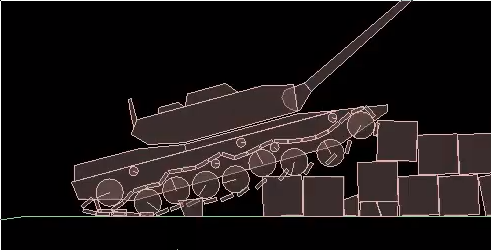
\includegraphics[width=10cm]{box2dDebug}
	\caption{Izrisovanje fizikalnih teles za potrebe razhroščevanja. Vir \cite{box2dTank}}
	\label{slika:box2dDebug}
\end{figure}

Unity podpira dva fizikalna pogona. Za 2D simulacijo ima integriran in razširjen Box2D, za 3D simulacijo pa modificiran PhysX. Uporaba fizikalnega pogona v Unity je zelo preprosta, saj našim objektom v igri dodamo komponento \textit{togo telo}. Unity v večini primerov poskrbi, da se konstrukcija sklada z izrisanim objektom in ponuja vizualno urejanje konstrukcije, če je to potrebno. Na sliki \ref{slika:unityRigidbody} vidimo primer dela s fizikalnim pogonom. Žoga, vidna na levi, prikazuje svojo konstrukcijo v zeleni barvi, na desni pa vidimo komponente igralnega objekta. Za fizikalno simulacijo sta pomembna \textit{konstrukcija krogle} () in \textit{RigidBody} (togo telo). Komponentam lahko nastavimo lastnosti konstrukcije in telesa, ki smo jih omenili zgoraj. V kodi lahko sledimo trkom v metodah \textit{OnTriggerEnter()} in \textit{OnCollissionEnter()}, ki nam podajo vse potrebne informacije o trkih, nakar lahko mi dodamo svojo kodo.

\begin{figure}[h]
	\centering
	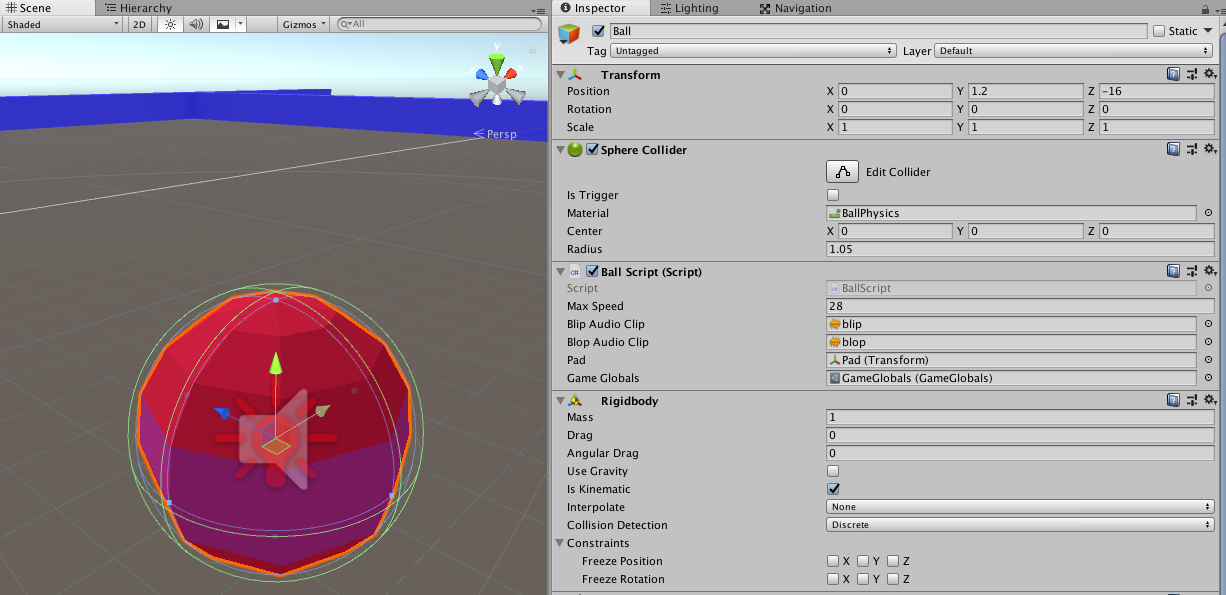
\includegraphics[width=15cm]{unityRigidbody}
	\caption{Urejanje konstrukcije in togega telesa na igralnem objektu}
	\label{slika:unityRigidbody}
\end{figure}

\subsection{Inteligenca v igrah}
Izraz inteligenca se v igrah uporablja za obnašanje vseh objektov, ki se odzivajo na svet in igralčeve akcije. Primeri inteligentnega obnašanja so: nasprotniki v igrah (se skrivajo za ovirami, poskušajo napasti igralce iz različnih smeri, se odzvati na igralčeve napade ipd.), prebivalci sveta (sledijo vsakodnevni življenjski rutini in se odzivajo na igralčeve akcije, kot je nasilje ali kraja) ipd. Z inteligenco poskusijo razvijalci obogatiti navidezni svet igre. Vendar uporabljena inteligenca v igrah (v komercialnih večjih igrah) ni umetna inteligenca, ki se uporablja na drugih področjih računalništva (ne-deterministične metode). Metode nevronskih mrež in genetskih algoritmov še ne doprinesejo rezultatov, ki bi igro naredile bolj zanimivo kot pa namenske metode \textit{umetne inteligence} v igrah. V akademskih krogih se veliko raziskuje vključevanja ne-determinističnih metod umetne inteligence v igre (v klasičnih igrah, kot so šah in go), vendar veliki studii še niso prestopili te meje. 

V igrah se tako uporabljajo deterministične metode, na katere lahko razvijalci sami vplivajo in jih priredijo za čim boljšo izkušnjo. Uporaba odločitvenih dreves, končnih avtomatov, mehke logike, iskanja poti in fiksno napisanih obnašanj je stalnica inteligence v igrah. Pri razvoju kompetentnih nasprotnikov omenjene metode niso vedno dovolj, zato se razvijalci poslužujejo goljufanja. Pri strateških igrah težji nasprotniki začnejo z več surovinami, lahko neskončno hitro izvajajo akcije in vedno vedo, kaj počne igralec in kje ima svojo vojsko.

Inteligenca v igrah je zelo široko področje, v našem delu smo zato opisali eno izmed najbolj uporabljenih metod iskanja poti. Ta se uporablja skoraj pri vseh naprednejših inteligencah v igrah. Kot zanimivost smo v repozitorij dodali članek kot dodatek magistrskemu delu, kjer smo uporabili genetski algoritem in poskusili prilagajati obnašanje nasprotnikov glede na akcije igralca. Članek je dostopen na povezavi \url{https://github.com/cimpresovec/Masters/blob/master/Thesis/LukaHorvatGenetski.pdf}.

\subsubsection{Algoritem A*}

A* in njegove izpeljanke so najbolj uporabljeni algoritmi iskanja najkrajše poti v igrah. Ker deluje na grafih, je uporaben za 2D in 3D igre. Razvijalci izdelajo grafe glede na stopnjo s čim manj vozlišči in ti so nato uporabljeni v algoritmu. A* je namenjen iskanju poti iz ene točke v drugo in temelji na algoritmu Dijkstra. Algoritem Dijkstra je metoda iskanja v globino po grafu, kjer se upoštevajo stroški prehoda med vozlišči in se tako prioritetno raziskuje najbolj obetavne poti. Tako dobimo usmerjen graf, po katerem lahko najbolj optimalno pridemo v katero koli vozlišče v grafu. A* doda dve pomembni spremembi. Prva je ta, da takoj, ko najdemo zaključno vozlišče, končamo iskanje in s tem preprečimo nepotrebno računanje, saj nas zanima le pot do cilja in ne celoten graf. Druga bolj pomembna sprememba pa je uvedba hevristike pri računanju prioritete vozlišč za raziskovanje. Prioriteta vozlišč pri Dijksta je odvisna od cene navigacije od začetnega vozlišča do trenutnega vozlišča. Pri A* tej prioriteti dodamo še ocenjeno razdaljo do končnega vozlišča. Ta razdalja je velikokrat kar evklidska razdalja po prostoru, neodvisno od ovir. Tako algoritem najprej raziskuje vozlišča, ki imajo do sedaj najmanjšo ceno od začetka poti in najmanjšo ocenjeno razdaljo do konca poti. 

Z zgoraj navedenimi spremembami izrazito izboljšamo hitrost iskanja poti po grafu, saj nas zanima samo pot do izbranega cilja. Pri igrah je zelo pomembna optimizacija grafov, saj je od tega odvisna hitrost delovanja algoritma. Grafe moramo prilagoditi stopnjam in obenem namenu uporabe. Če nas zanima samo najhitrejša navigacija po sobah v stavbi, potem postavimo samo eno vozlišče v vsako sobo in vrata. Če hočemo, da se nasprotnik pametno premika po sobi, pa moramo vključiti vozlišča glede na ovire po prostoru.

V programskih knjižnicah kot je RayLib moramo sami implementirati celotno rešitev iskanja poti, saj nam knjižnica ne ponuja nobene pomožne funkcionalnosti. LibGDX pa ponuja večji nabor funkcionalnosti za potrebe inteligence v igrah v paketu gdxAI, v katerem je vključen tudi A*. Ogrodje nam ponuja razrede za lažjo izgradnjo grafov in metode za preprosto uporabo algoritma. Poleg A* so v knjižnici na voljo še končni avtomati in odločitvena drevesa.

\subsubsection{Iskanje poti v Unity}

Unity ponuja širok spekter funkcionalnosti za iskanje poti. V ozadju implementira algoritem A*, vendar je glavna prednost pogona vsa dodatna funkcionalnost za lažjo uporabo. Iskanje poti v Unity uporablja štiri glavne komponente \cite{navmesh}:
\begin{itemize}
	\item \textbf{Navigacijska mreža (NavMesh)}. Predstavlja teren, po katerem se lahko premikajo objekti v naši igri. S pomočjo te komponente in algoritma za iskanje poti nam pogon išče optimalno pot iz točke A v točko B. Navigacijsko mrežo nam pogon ustvari sam iz objektov, ki jih označimo kot teren. Na sliki \ref{slika:navmesh} vidimo primer izdelave navigacijske mreže (obarvane z modro barvo). S parametri določimo lastnosti (višina in širina agenta, maksimalni naklon, dolžina možnega skoka in padca) nakar nam Unity ustvari mrežo na našem terenu (obarvan z belo barvo).
	\item \textbf{Agent navigacijske mreža (NavMesh Agent)}. Agenti so akterji, ki se premikajo po navigacijski mreži iz točke v točko. Obenem se izogibajo drugim agentom in oviram. Agenti lahko tako v igrah predstavljajo ljudi, avtomobile v mestih ipd.
	\item \textbf{Povezave mrež (Off-Mesh link)}. Če uporabljamo več navigacijskih mrež oziroma se v naših mrežah nahajajo luknje, potem z uporabo povezav določimo bližnjice, ki jih lahko uporabijo agenti med navigacijo. Recimo: agent lahko preskoči prepad ali skoči v globino, če so razdalje v mejah njegovih sposobnosti. Take bližnjice so vidne na sliki \ref{slika:navmesh}, kjer so predstavljene s povezanimi krogi.
	\item \textbf{Ovira navigacijske mreže (NavMesh Obstacle)}. Ovire so dinamični objekti, ki vplivajo na premike in navigacijo agentov. Če se ovira kotali proti agentu, se ji bo ta poskusil izogniti in nadaljevati svojo pot. Statična ovira spremeni samo navigacijsko mrežo, saj prekine prehodne dele in s tem spremeni izračun poti vsem agentov. 
\end{itemize}

\begin{figure}[h]
	\centering
	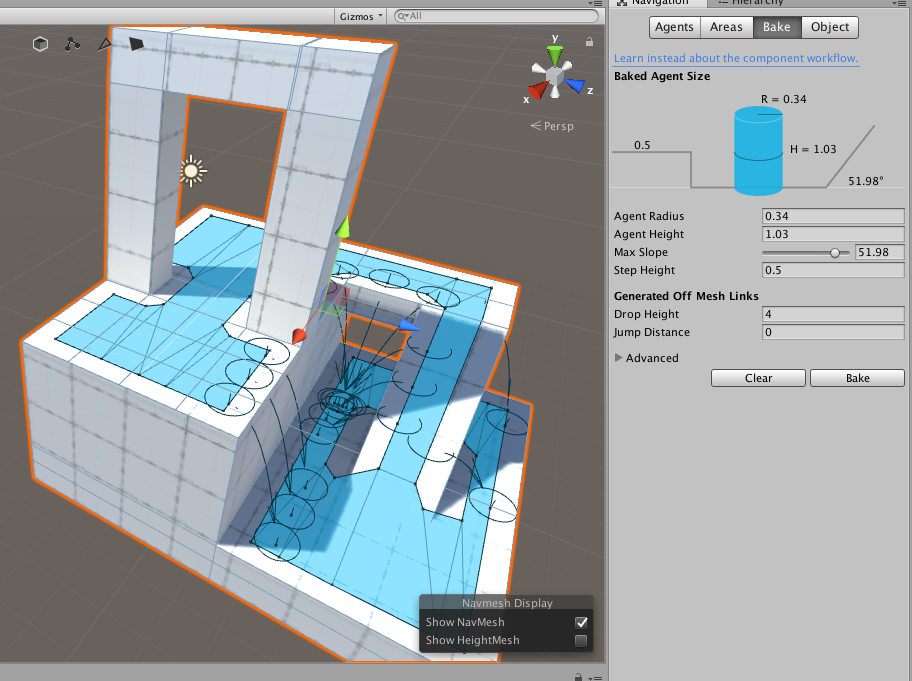
\includegraphics[width=15cm]{navmesh}
	\caption{Samodejna izgradnja navigacijske mreže v Unity.}
	\label{slika:navmesh}
\end{figure}

Uporaba navigacijskih komponent se proži iz kode na agentih navigacijske mreže. Agentu nastavimo lastnost \textit{destination} na vektor v prostoru, preostanek uredi pogon Unity. Dostop do poti po navigacijski mreži je na voljo preko lastnosti \textit{path} ali metode \textit{CalculatePath()}. Tako pridobimo vse točke navigacije po prostoru, katere lahko uporabimo za svojo logiko ali jih spremenimo in agentu nastavimo poljubno pot, če hočemo implementirati svoje obnašanje. 

\subsection{Unity ProBuilder}
Izdelava grafičnih gradnikov za nivoje in objekte v igri predstavlja večji del razvoja 3D iger. Večinoma se za to uporabljajo zunanja modelirna orodja, kot so Blender in Maya, vendar obstajajo alternativne rešitve za sam namenski pogon Unity. ProBuilder je ena izmed teh alternativ, ki v urejevalnik preko vtičnika doda širok nabor funkcionalnosti za urejanje. Vtičnik je bil v preteklosti plačljiv, vendar so ga odkupili Unity Technologies in ga integrirali v urejevalnik brez dodatnih licenc. Glavna prednost modeliranja v samem Unity urejevalniku je hitrejša iteracija gradnikov med razvojem. Pri zunanjih orodjih je potrebno model za vsako spremembo naložiti v orodju, ga popraviti in potem izvoziti za uporabo v projektu. S ProBuilder pa iteriramo na samih gradnikih v orodju, kjer lahko delamo spremembe celo medtem, ko se igra izvaja v urejevalniku.

Glavne funkcionalnosti ProBuilder-ja so:
\begin{itemize}
\item \textbf{Modeliranje.} Vse pomembne funkcije za delo z modeli so podprte. Lahko ustvarimo različne oblike osnovnih modelov (kocka, cilinder, krogla, stopnice, lok ipd.), urejamo oglišča, robove in ploskve, gladimo, uporabljamo triangulacijo, izruvanje, razdeljevanje ploskev ipd.
\item \textbf{Teksturiranje.} Izdelanim modelom lahko projiciramo UV koordinate in jih prirejamo po teksturi. Mogoče je tudi vizualno premikati teksturo po samem modelu v urejevalniku, da v trenutku vidimo končni rezultat.
\item \textbf{Barvanje oglišč.} Alternativa oziroma pomoč teksturiranju je barvanje posameznih oglišč. Z barvo oglišč lahko brez teksture izdelamo končni model ali vplivamo na teksturo, ki bo prekrivala. S tem lahko z eno teksturo na različnih modelih dosežemo variacije v odtenkih, kar skrajša potrebno delo.
\item \textbf{Integracija z drugo funkcionalnostjo pogona.} Izdelani modeli imajo avtomatsko pravilne konstrukcije za fizikalni pogon. Obenem je možno urejati navigacijske mreže za potrebe iskanja poti na izdelanih modelih.
\end{itemize}

Izdelane modele lahko tudi izvozimo za urejanje v zunanjih orodjih. Urejanje v pogonu se veliko uporablja pri prototipiranju igre, kjer uporabljamo preproste oblike in se ukvarjamo s postavitvami in oblikami stopenj. Po prototipu se velikokrat modeli izvozijo v zunanji program za podrobnejšo obdelavo. Odvisno od grafičnega stila igre pa se lahko odločimo, da vse gradnike izdelamo s ProBuilder-jem. 

Na sliki \ref{slika:probuilder} lahko vidimo uporabo vtičnika za izdelavo nivoja v igri. Na desni strani imamo na voljo različne funkcije za delo z modelom, v pogledu na levi pa urejamo posamezne ploskve v urejevalniku.

\begin{figure}[h]
	\centering
	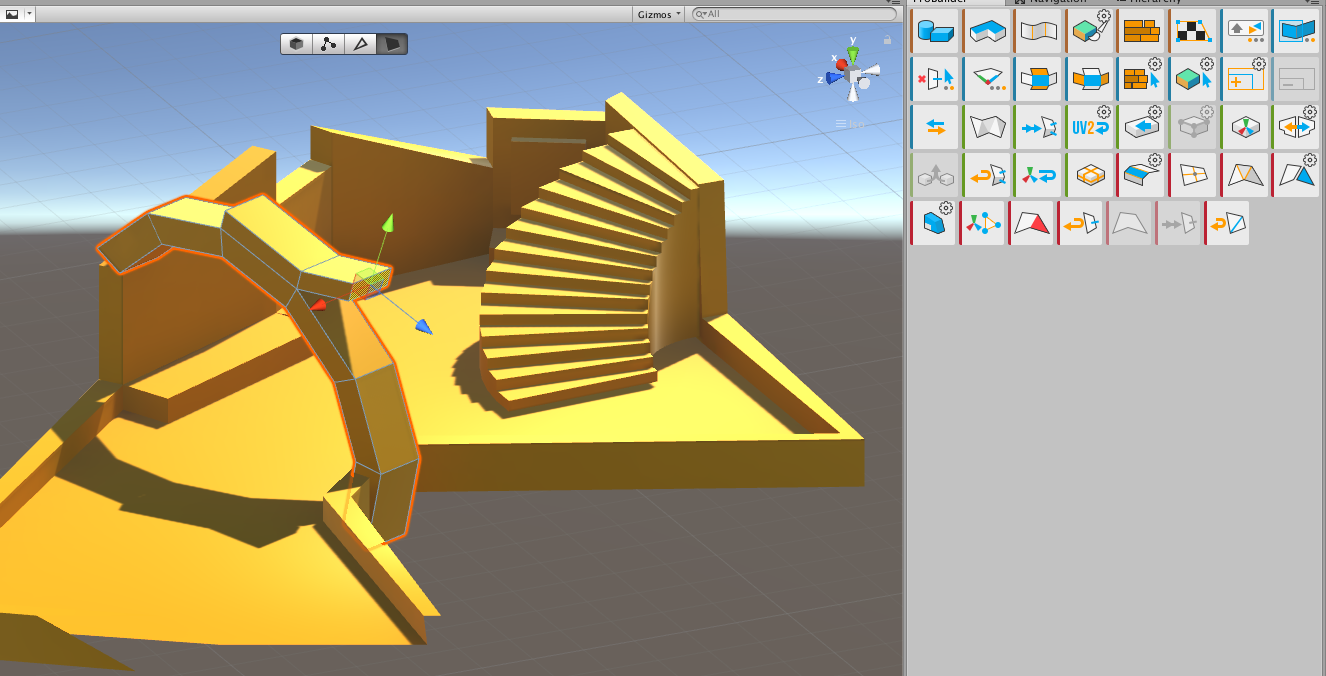
\includegraphics[width=15cm]{probuilder}
	\caption{Izdelava scene z ProBuilder vtičnikom v Unity}
	\label{slika:probuilder}
\end{figure}

\chapter{Analiza razvoja igre Breakout}\thispagestyle{fancy}
Razvoj igre Breakout je služil kot osnova za primerjavo treh različnih orodij za razvoj iger: knjižnica RayLib, ogrodje LibGDX in namenski pogon Unity. Skozi proces razvoja smo uporabljali opisane metode in prakse iz prejšnjih poglavjih. Glavni cilj je bil implementirati enako igro z enako funkcionalnostjo v vseh treh orodjih, vendar je prišlo zaradi ponujene funkcionalnosti v orodjih do specifičnih implementacijskih razlik:
\begin{itemize}
	\item Samo pogon Unity ponuja pomožno funkcionalnost za implementacijo začetnega zaslona z logotipom (začetni zaslon z Unity logotipom je obvezen pri brezplačni verziji pogona). Z nekaj kliki enostavno nastavimo željen osebni logotip, nakar pogon poskrbi za prikaz in prehod med scenami. Knjižnica RayLib in LibGDX take funkcionalnosti ne ponujata, zato smo morali sami implementirati začetni zaslon s transparentnim prehodom.
	\item Izgradnja glavnega menija se med orodji tehnološko zelo razlikuje. RayLib ne ponuja funkcionalnosti za izgradnjo grafičnega vmesnika, zato smo glavni meni zgradili s postavitvijo namenskih slik za gumbe in druge elemente. Tako smo morali sami paziti na pravilno postavitev elementov in prilagajanje po zaslonu. Klike na elemente smo morali ročno implementirati z zaznavanjem klika in položaja miške ob kliku.
	
	LibGDX ponuja pomožno funkcionalnost za izgradnjo grafičnih gradnikov, vendar potrebuje komponento \textit{Scene2D}. Obenem je postavljanje elementov opravljeno preko kode in ne ponuja grafičnega pomožnega orodja. Zato smo se pri LibGDX ogrodju odločili za podoben postopek kot pri knjižnici RayLib.
	
	Pogon Unity ponuja celotno funkcionalnost za izgradnjo grafičnih vmesnikov. Obenem je izgradnja vizualna v samem urejevalniku in temu primerno veliko enostavnejša. Unity Technologies je nedavno kupil namenski vtičnik imenovan TextMesh Pro, ki dodatno nadgradi zmožnosti izdelave vmesnikov in vtičnik vgradil v sam urejevalnik. Tako smo lahko preprosto zgradili hierarhijo glavnega menija igre, ki se dinamično prilagaja za različne ločljivosti igre. Obenem Unity ponuja enostavno programiranje odzivov na dogodke kot je klik na specifičen element vmesnika. Pogon tudi poskrbi za spreminjanje elementov, kadar klikamo po njih, kar nam prihrani pri izdelavi dodatnih grafičnih gradnikov.
	\item Implementacija glavnega dela igre (igranje stopenj) si je med orodji zelo podobna. Glavna razlika je pri delu s pogonom Unity, saj nam narekuje specifičen način dela, vendar je interna logika elementov igre vseeno dokaj podobna drugim orodjem. Največja razlika je način premikanja elementov (žoga, ovire in igralec) po prostoru. V RayLib in LibGDX smo sami skrbeli za delo z lokacijami, premikanjem in zaznavanjem trkov. V Unity pa smo uporabili fizikalni sistem za lažjo implementacijo. Vsi objekti imajo kinematična telesa in se premikajo z namenskimi metodami fizikalnega pogona. Za detekcijo trkov smo uporabili metode metanja žarkov in temu primerno sprožili odzive elementov.
	\item Kljub temu, da smo hoteli izdelati enako igro v vseh treh orodjih, pa nam je pogon Unity omogočal enostavno implementacijo dodatne funkcionalnosti v kratkem času. Tako smo ekskluzivno v pogonu Unity izdelali igro v 3D pogledu, saj je bilo potrebno samo zamenjati 2D grafične gradnike s 3D modeli ter premestiti kamero v prostoru. Obenem smo v igro dodali sistem luči in senc za lepšo grafično podobo igre. Pri uničevanju ovir smo tudi dodali, da te odletijo po prostoru s pomočjo dinamičnih fizikalnih teles.
\end{itemize}

Kot je razvidno iz zgoraj omenjenih razlik, je bila implementacija igre v pogonu Unity najlažja in najhitrejša. Časa izdelave v posameznih orodjih nismo merili, vendar si sledijo od najkrajšega do najdaljšega: pogon Unity, ogrodje LibGDX in knjižnica RayLib. Okvirno je izdelava v pogonu Unity bila enkrat hitrejša od knjižnice RayLib, saj nam pogon ponuja toliko več pomožne funkcionalnosti. Razlika je opazna tudi pri številu vrstic kode. Zavedamo se, da je število vrstic kode slaba metrika za primerjavo projektov, vendar smo jo vseeno vključili kot zanimivost. Analizo smo izvedli z brezplačnim orodjem \textit{cloc}:
\begin{itemize}
	\item Projekt z RayLib vsebuje 21 datotek z izvorno kodo ter 734 vrstic uporabne kode.
	\item Projekt z LibGDX vsebuje 9 datotek z izvorno kodo ter 630 vrstic uporabne kode.
	\item Projekt v Unity  vsebuje 9 datotek z izvorno kodo ter 257 vrstic uporabne kode.
\end{itemize} 

Knjižnica RayLib se je izkazala kot dobra mešanica nizkonivojske in visokonivojske knjižnice. Ponudila nam je večino funkcionalnosti, ki smo jih potrebovali za izdelavo igre. Obenem knjižnica ni vsiljevala nobenih vzorcev, tako da smo si lahko sami zastavili potrebno arhitekturo programske kode. Preprostost knjižnice pa je tudi njena slabost. Ko hočemo uporabiti katere izmed pogosteje uporabljenih metod in vzorcev, nam knjižnica večinoma ne ponuja nobene pomoči. Na primer ne nudi nobene pomoči za upravljanje stanj in gradnikov. Obenem ne ponuja pomoči pri vključevanju fizikalnega pogona in iskanja poti. Knjižnico priporočamo kot osnovo za izdelavo igre, če hočemo imeti večji nadzor nad arhitekturo in če raje sami implementiramo večino funkcionalnosti. Če hočemo hitrejši in preprostejši razvoj, potem knjižnice ne priporočamo, saj je potrebno več dela za samo implementacijo in integracijo bolj naprednih procesov. Knjižnica je še vedno v aktivnem razvoju in dopolnjevanju, zato upamo, da bo za pomanjkljivosti poskrbljeno v prihodnosti. 

Ogrodje LibGDX se je izkazalo kot vrhunec potrebne funkcionalnosti za razvoj iger brez uporabe namenskega pogona. Menimo, da na trgu ne obstaja visokonivojska knjižnica, ki ponuja toliko funkcionalnosti brez odvečnega vsiljevanja vzorcev v našo arhitekturo. Naslednji korak nad ogrodjem LibGDX so namenski pogoni, vendar se moramo takrat začeti prilagajati njemu, zato je LibGDX odlična izbira za izdelavo računalniških iger. Ponuja vso funkcionalnost, potrebno za vgraditev potrebnih principov in metod razvoja iger, obenem pa ponuja tudi pomoč pri vključevanju kompleksnejših metod, kot je fizikalni pogon. Je tudi preprosta za razširitev, če hočemo spremeniti obnašanje osnovne funkcionalnosti. Ogrodje priporočamo kot vstopno točko za vse, ki ne rabijo najnovejše tehnologije, ki jo ponujajo namenski pogoni. Glavno pomanjkljivost vidimo v upočasnjenem razvoju ogrodja, saj avtor več aktivno ne sodeluje pri razvoju in je delo prevzela preostala skupnost.

Namenski pogon Unity ponuja vse, kar potrebujemo za razvoj računalniških iger od malih individualnih projektov do komercialnih iger večjih studiov. Pogon ponuja preprosto uporabo z vizualnim urejevalnikom, veliko skupnostjo, polno navodil in pomoči ter najnovejšo tehnologijo za potrebe razvoja. Obenem je med vsemi opisanimi orodji najpreprostejši za uporabo za novince, večinoma zaradi manjše potrebe znanja programiranja in večjim poudarkom na vizualnem delu. Največjo slabost pogona vidimo v večji končni velikosti iger (pri manjših projektih se to hitro pozna) ter arhitekturo projekta, ki ga pogon vsili z njegovo uporabo. Pogon priporočamo vsem, ki jih ne moti prilagoditi se na način dela s pogonom ter tistim, ki nimajo izkušenj z izdelavo iger. Nadaljnji razvoj pogona je videti obetaven, saj se razvijalci trudijo korenito izboljšati največje slabosti pogona v bližnji prihodnosti.

Kot omenjeno so vsi projekti na voljo na GitHub repozitoriju na naslednji povezavi: \url{https://github.com/cimpresovec/Masters}. Projekt ima MIT licenco in vsebuje vso vsebino, izdelano za potrebe tega magistrskega dela.

\chapter{Sklep}\thispagestyle{fancy}
V magistrskem delu smo predstavili potreben nabor orodij, postopkov in metod za izdelavo računalniške igre. Kot demonstracijo teh orodij smo implementirali računalniško igro v C++ z RayLib, Javi z LibGDX in v pogonu Unity. Obenem smo izdelali potrebne grafične gradnike z orodjema Inkscape za 2D grafiko in orodjem Blender za 3D grafiko. Zvočne gradnike smo izdelali z orodjem BFXR.

Grafični gradniki so preprostih oblik, vendar služijo svojemu namenu za predstavitev posameznih objektov. Največjo pomanjkljivost gradnikov vidimo v 3D modelih, saj nismo imeli dovolj izkušenj za izdelavo bolj podrobnih in kakovostnih modelov. Potrebne modele bi bilo možno pridobiti s spleta, vendar smo za potrebe magistrskega dela sami preučili metode in izdelali gradnike. Pri zvočnih gradnikih nismo sami izdelali glasbe, ampak smo s spleta pridobili javno dostopno skladbo za igro. Pri tem je bila največja težava poznavanje potrebne glasbene teorije in izkušnje, ki so potrebne za izdelavo takih gradnikov.

Z implementiranimi igrami smo predstavili najpomembnejše prakse in metode v treh različnih orodjih. Obenem smo primerjali ponujene možnosti za implementacijo med orodji in metode opisali v magistrskem delu. Implementirana igra je implementacija arkadne igre Breakout, vendar ta ni bila namen dela. Namen dela so bili uporabljeni postopki, ki so neodvisni od projekta. S kompleksnejšo igro bi lahko predstavili več naprednih praks, katerih nismo obdelali v sklopu magistrskega dela.

Implementirane igre smo med sabo analizirali v smislu implementacijskih razlik in prišli do končnih ocen oziroma sklepov o posameznih uporabljenih orodjih. Knjižnica RayLib nam je ponujala veliko svobode pri uporabi njene funkcionalnosti, vendar ni zadostovala potrebam implementacije naprednejših funkcionalnosti. Izkazala se je kot odlična vstopna točka za poučne projekte, kjer je cilj implementirati večji del funkcionalnosti ročno. Ogrodje LibGDX se je izkazalo za najboljšo izbiro za projekte vseh obsežnosti, ki hočejo biti neodvisni od večjih namenskih pogonov, kot so Unity in Unreal Engine. Ponujalo je prostost uporabe kot knjižnica RayLib, vendar dodalo velik nabor potrebne dodatne funkcionalnosti. Pogon Unity nam je ponudil vse potrebno funkcionalnost in še veliko več za potrebe razvoja iger. Hitreje in enostavneje smo implementirali enako oziroma boljšo funkcionalnost kot v drugih orodjih. Pogon priporočamo vsem, ki potrebujejo celotni paket funkcionalnosti za razvoj in jih ne moti prilagajanje podanim konvencijam.

Uspešno smo predstavili ves potreben nabor orodij in praks, ki so potrebne za izdelavo računalniške igre. Obdelali smo le najbolj pogosto uporabljene metode in tri glavna orodja za tehnično implementacijo. V nadaljnjih delih bi se lahko osredotočili na bolj napredne sklope razvoja iger, kot so igre za več igralcev, proceduralne metode v igrah ipd. Obenem bi lahko pokrili še preostala večja orodja na trgu, kot so Unreal Engine in preostale ogleda vredne projekte, kot je Godot. Vsekakor mislimo, da smo pokrili potrebno področje, ki bo posameznika popeljalo v svet razvoja računalniških iger.

\cleardoublepage
\addcontentsline{toc}{chapter}{Literatura}
\bibliographystyle{plain}
\bibliography{thesis}

\end{document}